\documentclass[twocolumn,traditabstract]{aa}  
\usepackage{fixltx2e}
\usepackage[english]{babel}
\usepackage{graphicx,amsmath}
%\usepackage{epstopdf}
\usepackage{epsf,color}
\usepackage[mathscr]{eucal}
\usepackage{amsmath}
\usepackage{amssymb,amsfonts}
\usepackage{natbib}
\usepackage{txfonts}
\usepackage{dsfont}
\definecolor{Mygreen}{rgb}{0.00, 0.72, 0.0}
\definecolor{Mypink}{rgb}{1.0, 0.0, 0.5}
\usepackage[breaklinks, citecolor=blue, linkcolor=Mygreen, urlcolor=Mypink, colorlinks=true, debug, baseurl=' ']{hyperref}
\usepackage{float}
\usepackage{color}
%\usepackage{scrextend}
%\usepackage{nccmath}
%\usepackage{mathtools, cuted}
%\usepackage{lscape}
\usepackage{widetext}
%\usepackage{flushend}
%\usepackage[T1]{fontenc}


\newcommand{\nika}{{\it NIKA}}
\newcommand{\nikad}{{\it NIKA2}}


\def\intk#1{\displaystyle\int\frac{d^2k_{#1}}{(2\pi)^2}}
\def\intr#1{\displaystyle\int d^2r_{#1}}
\def\simlt{\lower.5ex\hbox{$\; \buildrel < \over \sim \;$}}
\def\simgt{\lower.5ex\hbox{$\; \buildrel $\textgreater$ \over \sim \;$}}
\def\NIKA{\textit{NIKA}}
\def\NIKAd{\textit{NIKA2}}
\def\Archeops{\textit{Archeops}}
\def\Planck{\textit{Planck}}
\def\WMAP{\textit{WMAP}}
\def\Skydip{\textit{Skydip}}

\bibpunct{(}{)}{;}{a}{}{,}
\bibliographystyle{aa}

\begin{document}
\title{Crab nebula polarization observations with NIKA: \\ implications for future CMB experiments}
%\author{A.~Ritacco \inst{\ref{LPSC}}\thanks{Corresponding author: Alessia Ritacco, \url{ritacco@lpsc.in2p3.fr}}
\and  N.~Ponthieu \inst{\ref{IPAG}}
\and  A.~Catalano \inst{\ref{LPSC}}
\and R.~Adam \inst{\ref{LPSC},\ref{OCA}}
\and  P.~Ade \inst{\ref{Cardiff}}
\and  P.~Andr\'e \inst{\ref{CEA}}
\and  A.~Beelen \inst{\ref{IAS}}
\and  A.~Beno\^it \inst{\ref{Neel}}
\and  A.~Bideaud \inst{\ref{Neel}}
\and  N.~Billot \inst{\ref{IRAME}}
\and  O.~Bourrion \inst{\ref{LPSC}}
\and  M.~Calvo \inst{\ref{Neel}}
\and  G.~Coiffard \inst{\ref{IRAMF}}
\and  B.~Comis \inst{\ref{LPSC}}
\and  F.-X.~D\'esert \inst{\ref{IPAG}}
\and  S.~Doyle \inst{\ref{Cardiff}}
\and  J.~Goupy \inst{\ref{Neel}}
\and  C.~Kramer \inst{\ref{IRAME}}
\and  S.~Leclercq \inst{\ref{IRAMF}}
\and  J.F.~Mac\'ias-P\'erez \inst{\ref{LPSC}}
\and  P.~Mauskopf \inst{\ref{Cardiff},\ref{Arizona}}
\and A. Maury \inst{\ref{CEA}}
\and  F.~Mayet \inst{\ref{LPSC}}
\and  A.~Monfardini \inst{\ref{Neel}}
\and  F.~Pajot \inst{\ref{IAS}}
\and  E.~Pascale \inst{\ref{Cardiff}}
\and  L.~Perotto \inst{\ref{LPSC}}
\and  G.~Pisano \inst{\ref{Cardiff}}
\and M.~Rebolo-Iglesias  \inst{\ref{LPSC}}
\and  V.~Rev\'eret \inst{\ref{CEA}}
\and  L.~Rodriguez \inst{\ref{CEA}}
\and  C.~Romero \inst{\ref{IRAMF}}
\and F.~Ruppin \inst{\ref{LPSC}}
\and G.~Savini \inst{\ref{London_college}}
\and  K.~Schuster \inst{\ref{IRAMF}}
\and  A.~Sievers \inst{\ref{IRAME}}
\and C. Thum \inst{\ref{IRAME}}
\and  S.~Triqueneaux \inst{\ref{Neel}}
\and  C.~Tucker \inst{\ref{Cardiff}}
\and  R.~Zylka \inst{\ref{IRAMF}}}

%\institute{
Laboratoire de Physique Subatomique et de Cosmologie, Universit\'e Grenoble Alpes, CNRS/IN2P3, 53, avenue des Martyrs, Grenoble, France
  \label{LPSC}
  \and
  Laboratoire Lagrange, Universit\'e C\^ote d'Azur, Observatoire de la C\^ote d'Azur, CNRS, Blvd de l'Observatoire, CS 34229, 06304 Nice cedex 4, France
  \label{OCA}
  \and
Institut de RadioAstronomie Millim\'etrique (IRAM), Grenoble, France
  \label{IRAMF}
\and
Laboratoire AIM, CEA/IRFU, CNRS/INSU, Universit\'e Paris Diderot, CEA-Saclay, 91191 Gif-Sur-Yvette, France 
  \label{CEA}
\and
Astronomy Instrumentation Group, University of Cardiff, UK
  \label{Cardiff}
\and
Institut d'Astrophysique Spatiale (IAS), CNRS and Universit\'e Paris Sud, Orsay, France
  \label{IAS}
\and
Institut N\'eel, CNRS and Universit\'e Grenoble Alpes, France
  \label{Neel}
\and
Institut de RadioAstronomie Millim\'etrique (IRAM), Granada, Spain
  \label{IRAME}
\and
Dipartimento di Fisica, Sapienza Universit\`a di Roma, Piazzale Aldo Moro 5, I-00185 Roma, Italy
  \label{Roma}
\and
Univ. Grenoble Alpes, CNRS, IPAG, F-38000 Grenoble, France 
  \label{IPAG}
    \and
Aix Marseille Universit\'e, CNRS, LAM (Laboratoire d'Astrophysique de Marseille) UMR 7326, 13388, Marseille, France
  \label{LAM}
\and
School of Earth and Space Exploration and Department of Physics, Arizona State University, Tempe, AZ 85287
  \label{Arizona}
\and
Universit\'e de Toulouse, UPS-OMP, Institut de Recherche en Astrophysique et Plan\'etologie (IRAP), Toulouse, France
  \label{IRAP}
\and
CNRS, IRAP, 9 Av. colonel Roche, BP 44346, F-31028 Toulouse cedex 4, France 
  \label{IRAP2}
\and
University College London, Department of Physics and Astronomy, Gower Street, London WC1E 6BT, UK
  \label{UCL}
\and 
Institut d'Astrophysique de Paris, CNRS (UMR7095), 98 bis boulevard Arago, F-75014, Paris, France
  \label{IAP}
\and 
LERMA, CNRS, Observatoire de Paris, 61 avenue de l'Observatoire, Paris, France
  \label{LERMA}
}

\date{Received \today \ / Accepted --}
	
\abstract{The detection of the primordial CMB B-modes in polarization constitutes one of the major challenges of modern cosmology. Their precise measurement requires accurate determination of foreground contaminants as well as of the absolute calibration of the instrument in terms of cross polarization and absolute polarization angle reconstruction. We  present here a study of the Crab nebula, which is a well known polarization angle calibration source. The Crab nebula is the most intense source in the microwave sky with an extension of few arcminutes corresponding to the typical beamwidth of current CMB experiments. The Crab nebula exhibits a highly polarized synchrotron radiation at radio and millimeter wavelengths. 
We report in this paper high resolution (18$^{\prime\prime}$ FWHM) observations of the Crab nebula in intensity and polarization at 150 GHz with the \NIKA\ camera.
\NIKA, operated at the IRAM 30 m telescope from 2012 to 2015, is a camera made of Lumped Element Kinetic Inductance Detectors (LEKIDs) observing the sky at 150 and 260 GHz. 
 From these observations we are able to reconstruct the spatial distribution of the Crab nebular polarization degree and angle, which is found to be compatible with previous observations at lower and higher frequencies. 
Averaging across the source and using other existing data sets we find that the Crab nebula polarization angle is consistent with being constant across frequencies with a value of $ -88.1 \pm 0.3$.  
We also present the first estimation of the Crab nebula Spectral Energy Distribution in polarization.  These measurements will be of interest for current and next generation of CMB experiments operating at (sub)-mm and mm wavelengths. }
\titlerunning{NIKA polarisation observations of the Crab nebula.}	
\authorrunning{A. Ritacco, J. F. Mac\'ias P\'erez , N. Ponthieu et al.}
\keywords{Techniques: polarization -- KIDs --  individual: NIKA }
\maketitle
\begin{figure*}[h!]
  \centering
     	  { 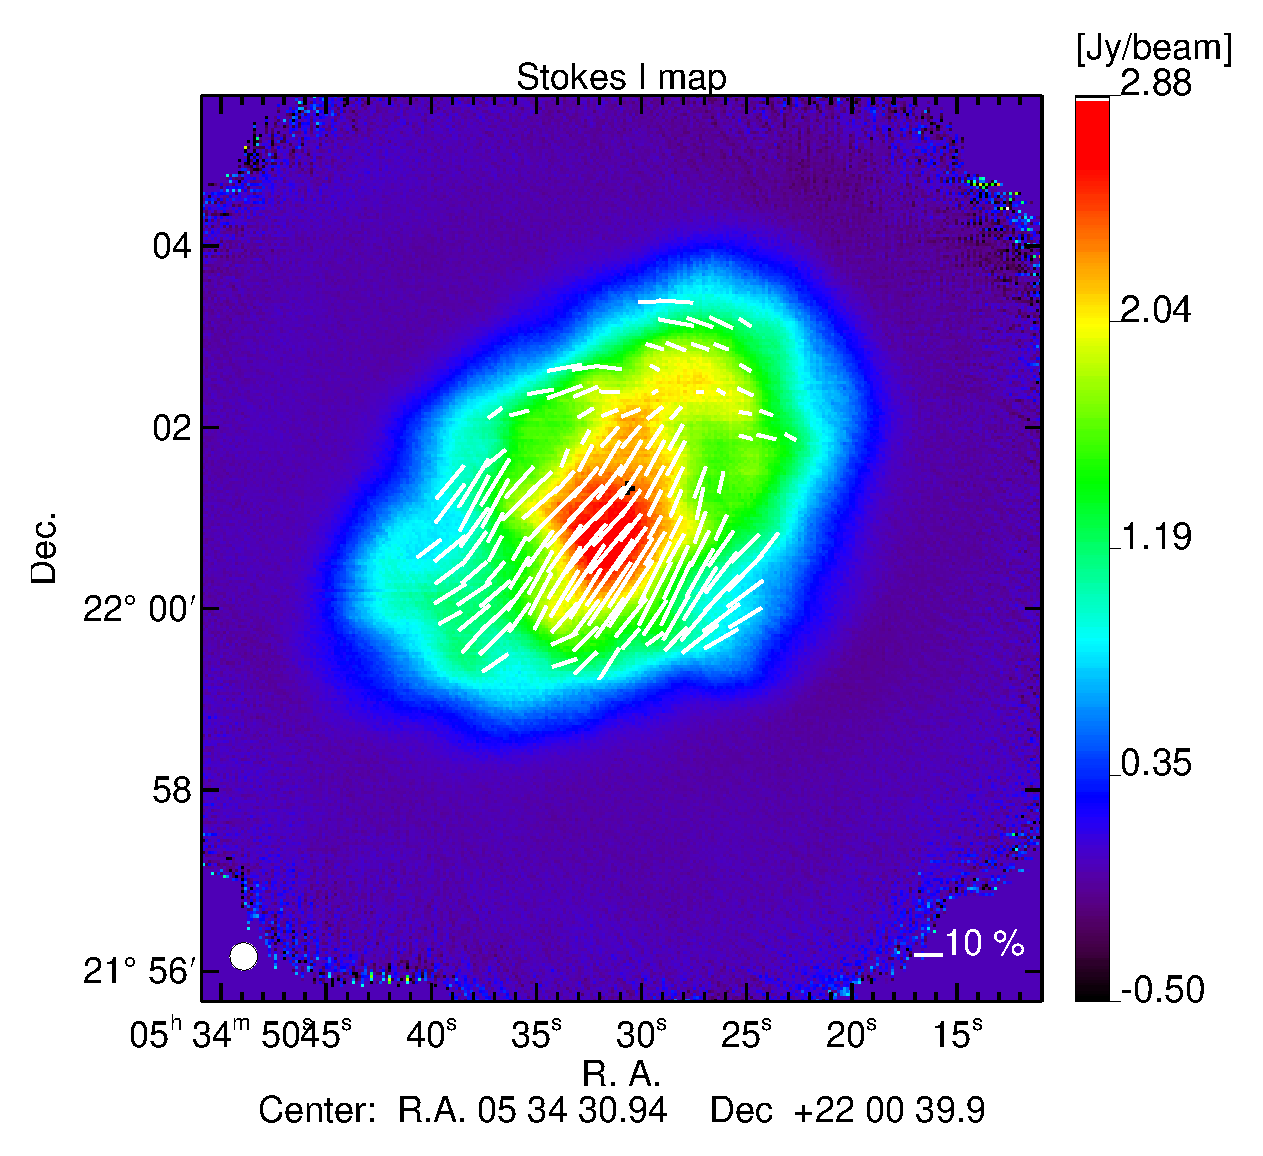
\includegraphics[width=0.32\linewidth,keepaspectratio]{figures/Crab_I_map2_2mm.pdf}}	
	     { 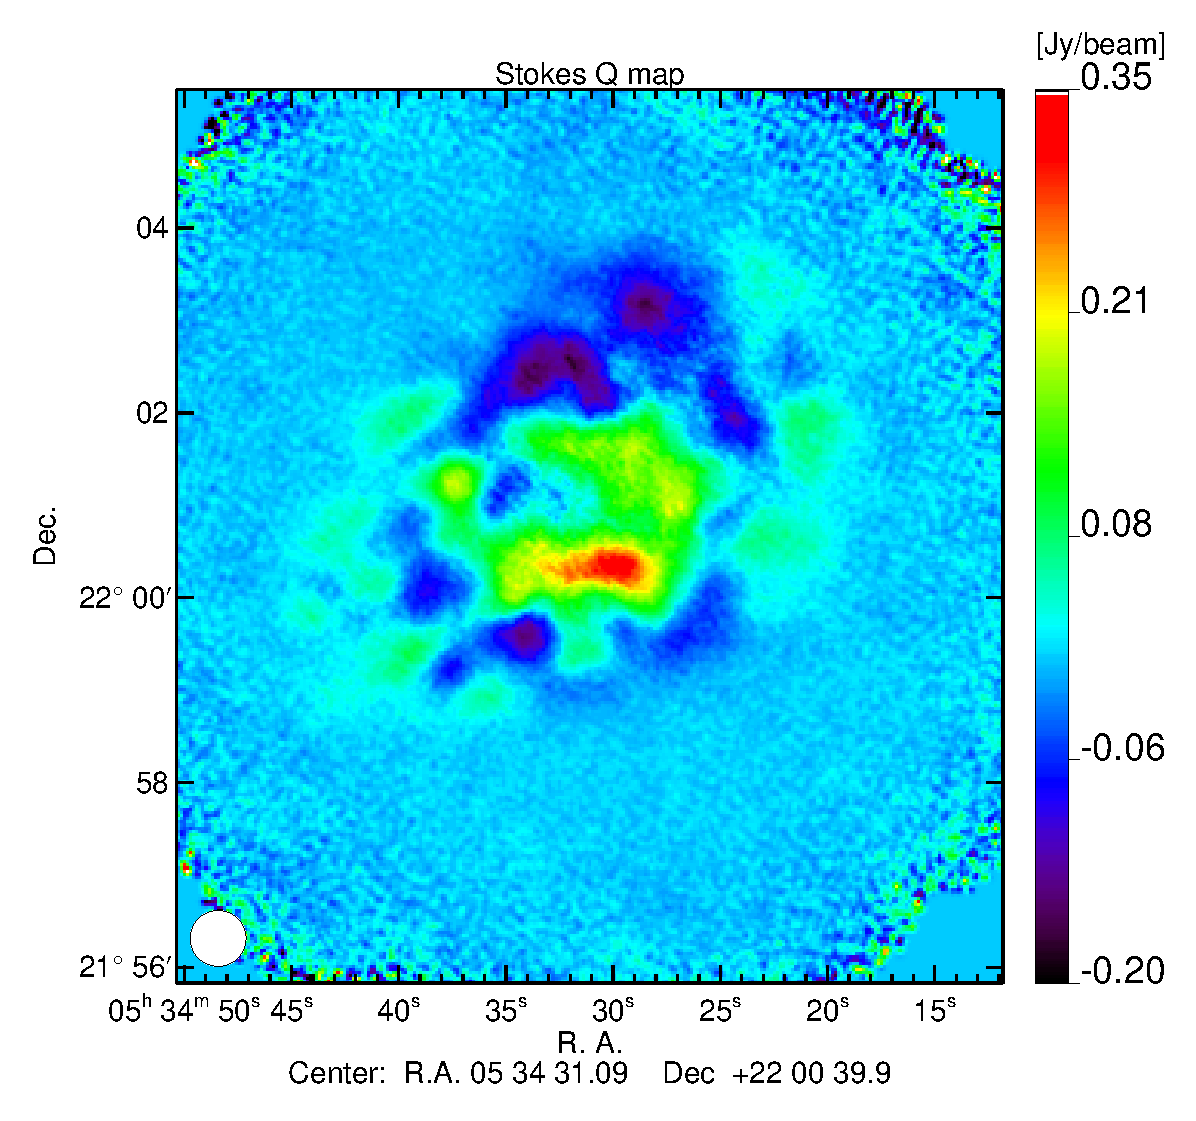
\includegraphics[width=0.32\linewidth,keepaspectratio]{figures/Crab_Q_map2_2mm.pdf}}
          { 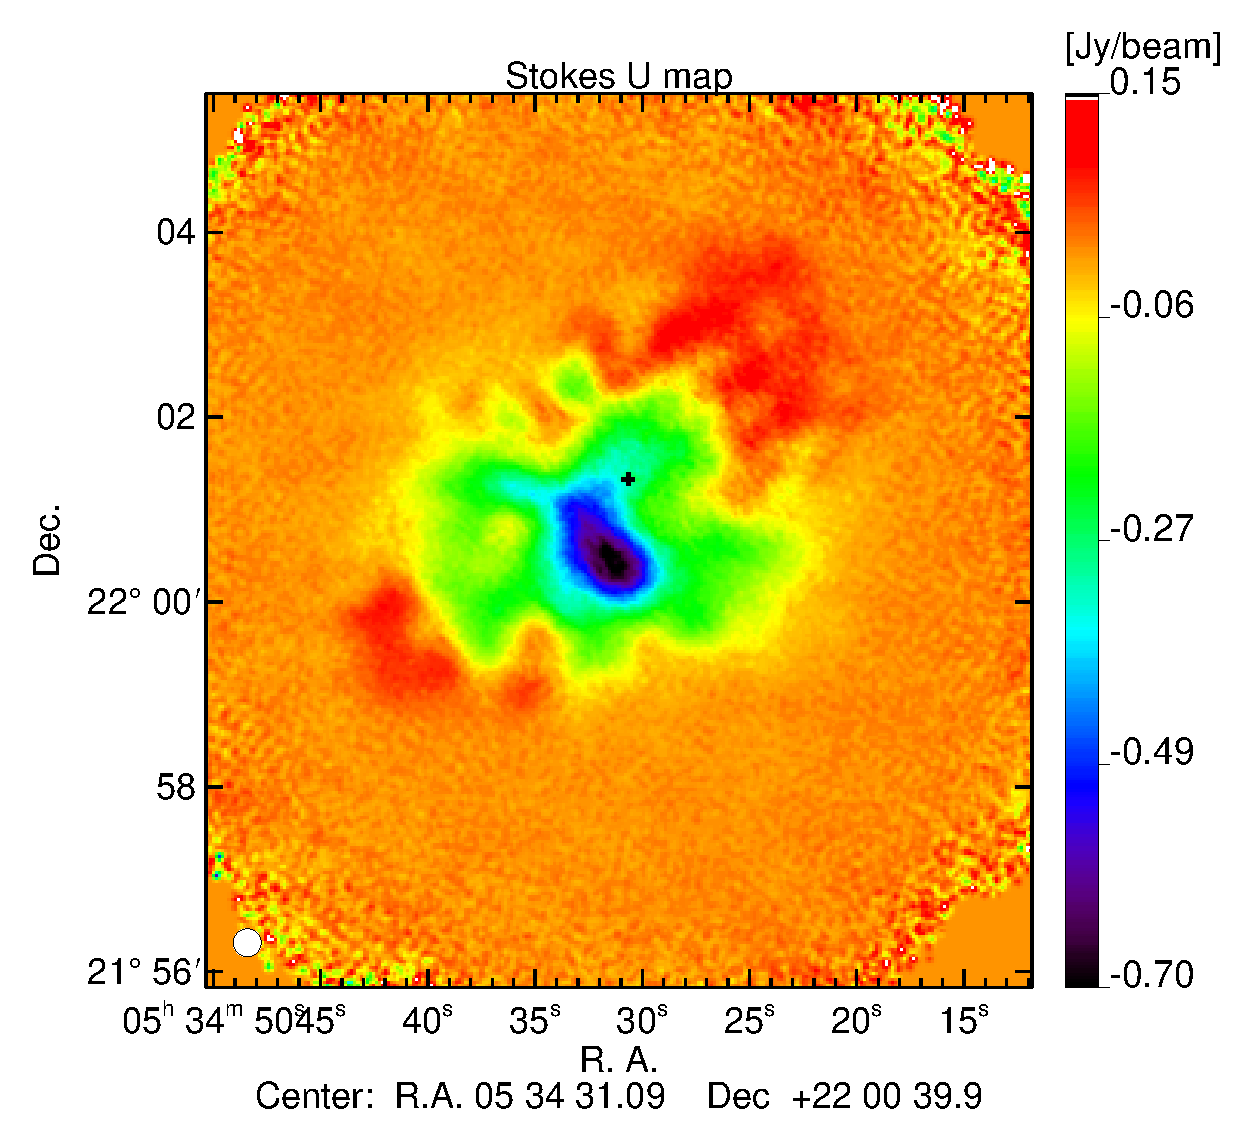
\includegraphics[width=0.32\linewidth,keepaspectratio]{figures/Crab_U_map2_2mm.pdf}} 
           \caption{From left to right: Crab nebula Stokes $I$, $Q$ and, $U$ maps obtained at 150 GHz with the \NIKA\ camera. Polarization vectors, indicating both the degree and the orientation, are over-plotted in black on the intensity map where the polarization intensity satisfies P $\textgreater$  3 $\sigma_P$, where $\sigma_P$ represents the uncertainty in P. }
\label{crab_intensity_maps}
\end{figure*}


\section{Introduction}\label{sec:introduction}
The polarization of the Cosmic Microwave Background (CMB) anisotropies offers a powerful way to investigate the early Universe. They can be decomposed into a scalar and a pseudo-scalar field, respectively called $E$  and $B$ modes. The primordial density fluctuations (scalar perturbations) can only produce $E$ CMB polarization, while $B$ CMB polarization can only be produced by 
primordial (tensor perturbations) gravitational waves \citep{polnarev1985polarization, 1997PhRvL..78.2054S} arising from the inflationary epoch \citep{PhysRevD.23.347, linde1982new} and by gravitational lensing of the $E-$modes \citep{ade2015planck}.
The detection of the primordial $B-$modes could definitively probe the existence of an inflationary epoch and constitutes one of the most ambitious goals of modern observational cosmology.

Recently, \citet{bicepplanck2015,bicep2016} set a 95\% upper limit for the detection of the tensor to scalar ratio $r$ $\textless$ 0.07.
Upcoming CMB experiments aiming at measuring the primordial $B-$modes require an accurate determination of the foreground emissions to the CMB signal and a high control of the systematic effects. One of the most difficult parameters to be characterized for a CMB polarization experiment is the calibration of residual cross polarization and of the absolute polarization angle. This can be achieved using observations of well known polarized sources like the Crab nebula.

The Crab Nebula (or Tau A) located at equatorial coordinates $R.A. = 5^h34^m32s$ and $Dec. = 22^{\circ}0^{\prime}52^{\prime\prime}$ is a plerion-type supernova remnant emitting a highly polarized signal \citep{1978A&A....70..419W,1991ApJ...368..463M}.
A synchrotron emission from the nebula is observed in the radio frequency domain, which is powered by a pulsar through its jet. 
Moreover, near the center of the nebula we observe a shock, which is formed where the jet is thermalized and ultra-relativistic particles are released into the surrounding nebula \citep{2000ApJ...536L..81W,2011A&A...528A..11W}. 

The Crab nebula is the most intense polarized astrophysical object in the microwave sky at angular scales of few arcminutes and for this reason it is of particular interest  for the calibration of CMB polarization experiments, which have beamwidths comparable to the extension of the source.
For a more detailed review on this source we refer to \citet{2008ARA&A..46..127H}.

The Crab nebula is used for polarization cross-check analysis in the frequency range from 30 to 353 GHz \citep{2011ApJS..192...19W,2015arXiv150702058P}. High angular resolution observations from the XPOL experiment \citep{thum2008} at the IRAM 30 m telescope have revealed the spatial distribution of the Crab Nebula in intensity and polarization at 90 GHz with an absolute accuracy of 0.5$^{\circ}$ in the polarization angle \citep{aumont2010}. 
This kind of high angular resolution observations of the Crab nebula in polarization could be very useful for the calibration of the next generation of polarization experiments. In particular those aiming at a precise measurement of the CMB polarization, which have a large frequency range to be able to carefully study and subtract foreground emission \citep{2016IJMPD..2540008K}. 

Previous studies \citep{macias2010} of the total Spectral Energy Distribution (SED) of the Crab nebula have shown a spectrum well described by a single synchrotron component at radio and mm wavelengths, and predict negligible variations in polarization fraction and angle in the frequency range of interest for CMB studies.
 
Polarized observations of the Crab Nebula have been performed with the \NIKA\ camera \citep{monfardini2010,catalano2014,monfardini2014} at the IRAM 30 m telescope during the observational campaign of February, 2015. A first overview in \NIKA\ Crab polarization observations was given in \cite{2016JLTP..184..724R}. In this paper we go a step forward in the analysis and combine the \NIKA\ observations with previous ones
in order to trace the polarized SED of the Crab nebula. We use polarization observations from the WMAP satellite at 23, 33, 41, 61 and 94 GHz \citep{2011ApJS..192...19W}, from the \Planck\ satellite at 30, 44, 70, 100, 143, 217, 353 GHz and from XPOL at 90 GHz \citep{aumont2010}. 
 The paper is organized as follows: in Sec.~\ref{sec:NIKA observations} the intensity and polarization maps obtained with the \NIKA\ camera are presented together with the polarization degree and angle spatial distributions; Sec.~\ref{sec:Polarization estimates in CMB experiments like beams} presents the reconstruction of the polarization properties of the Crab nebula in well defined regions; Sec.~\ref{sec:Polarization intensity Spectral Energy Density (SED)} presents the Crab nebula SED in temperature and polarization; in Sec.~\ref{sec:conclusions} we draw conclusions.
 \begin{figure*}
\centering
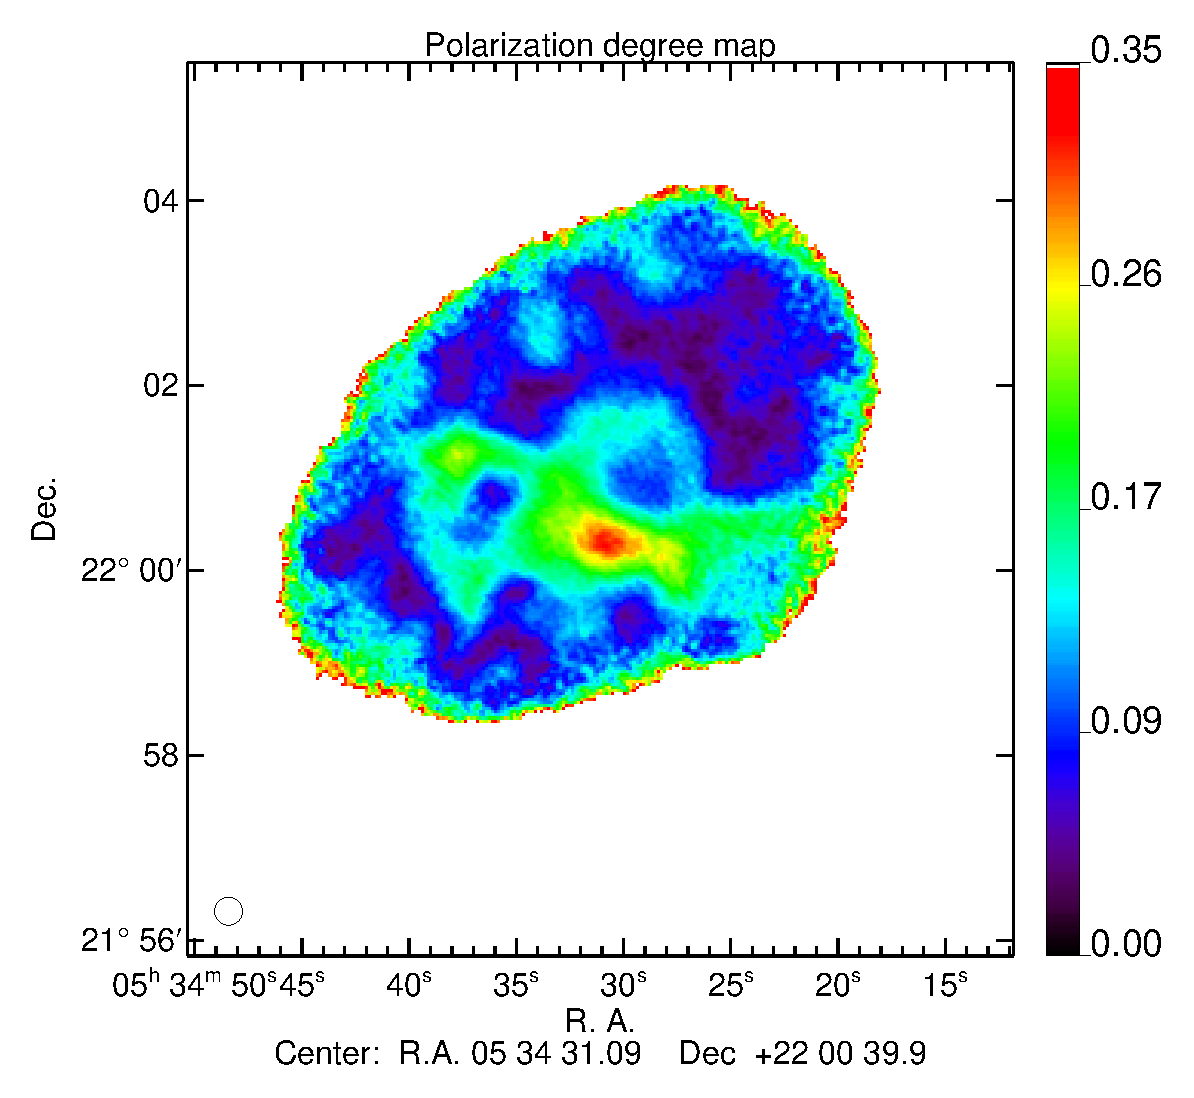
\includegraphics[clip, angle=0, scale = 0.35]{figures/Crab_pol_deg2_2mm.pdf}
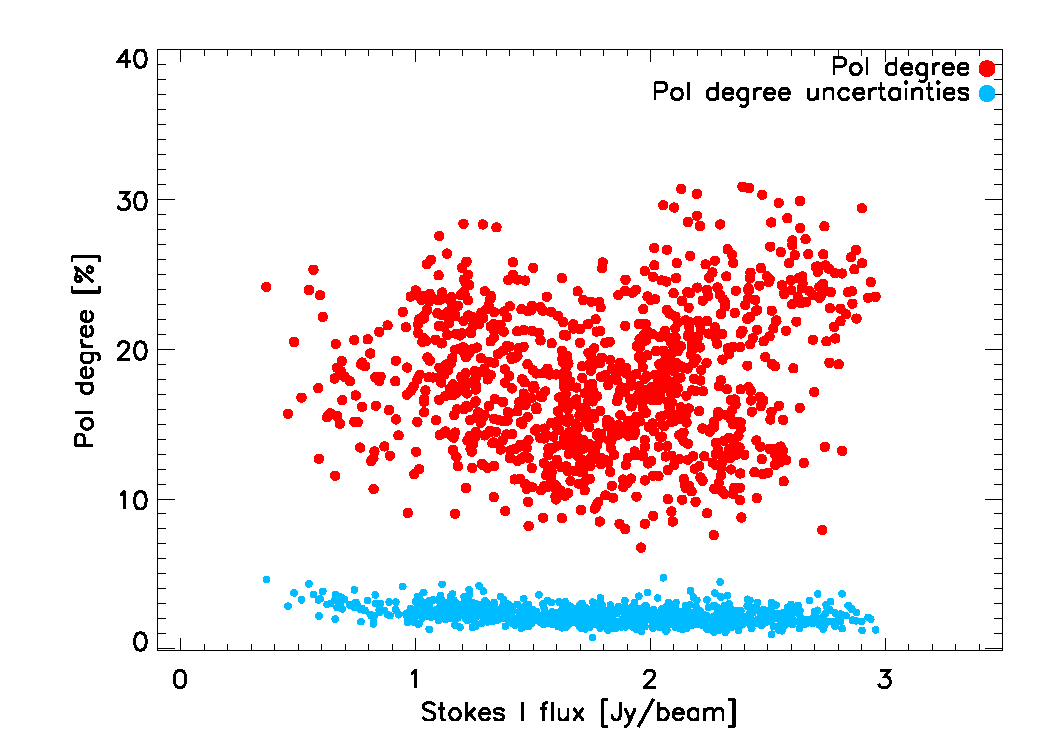
\includegraphics[clip, angle=0, scale = 0.5]{figures/pol_deg_vs_I_2mm.pdf}
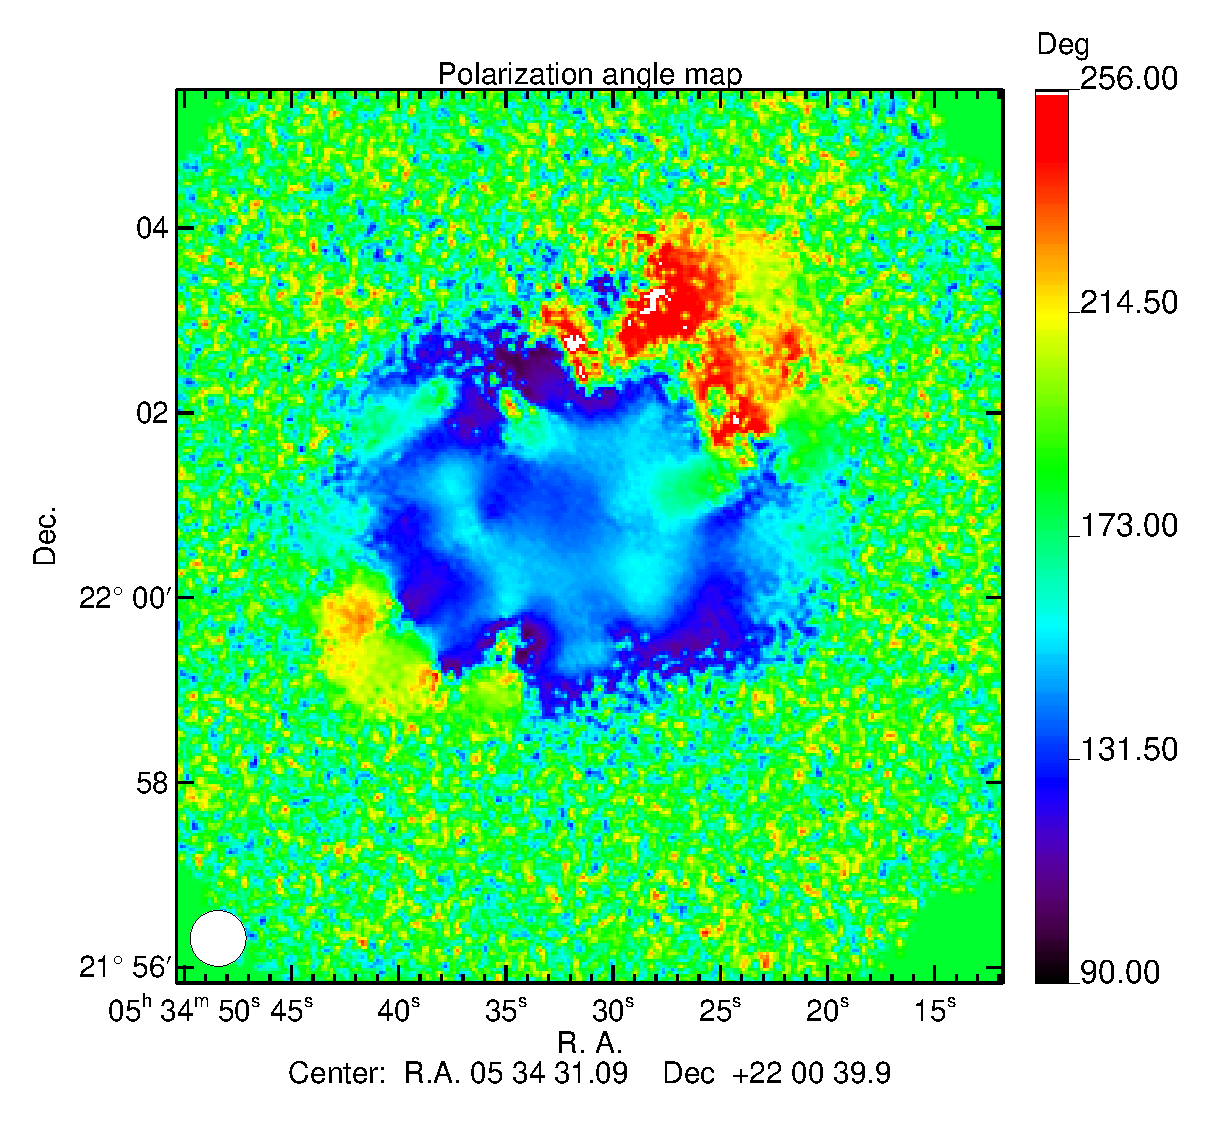
\includegraphics[clip, angle=0, scale = 0.35]{figures/Crab_angle2_2mm.pdf}
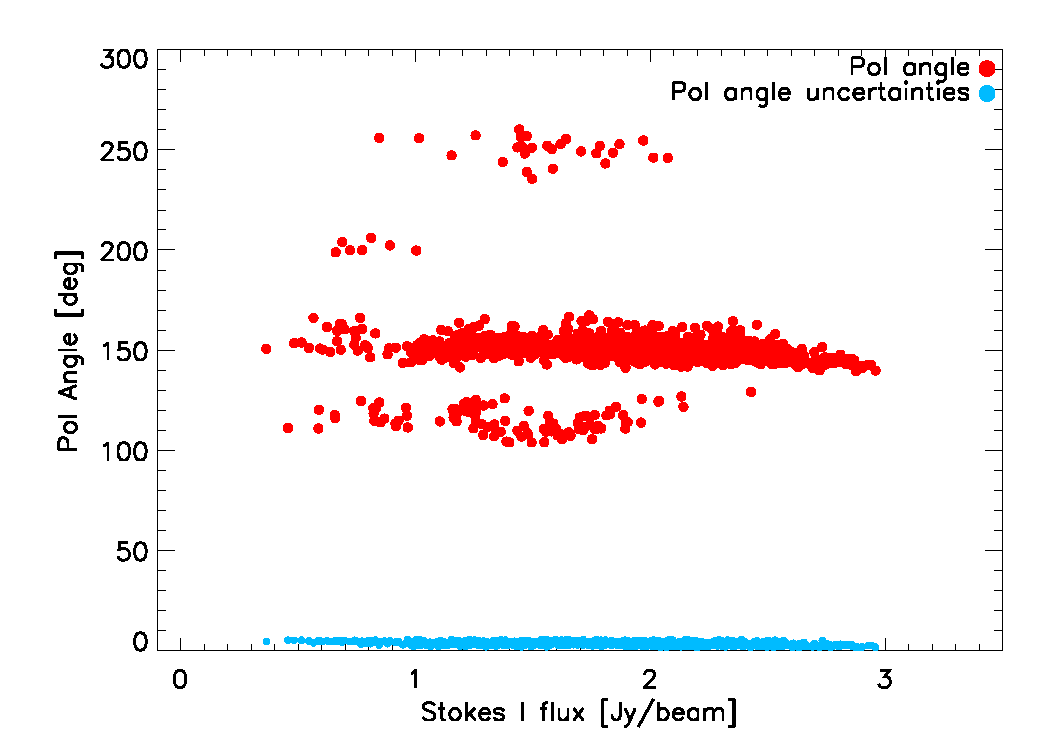
\includegraphics[clip, angle=0, scale = 0.5]{figures/pol_angle_vs_I_2mm.pdf}
\caption{{\it Top}: noise bias uncorrected polarization degree map $p$ (left) of the Crab nebula. The right panel shows the noise bias corrected $p$ values as a function of total intensity map (Stokes $I$). The condition $P$ $\textgreater$ 5$\sigma_{P}$ is satisfied for those values. {\it Bottom}: polarization angle map $\psi$ (left) of the Crab nebula. On the right panel the distribution of $\psi$ values is represented as a function of the total intensity where $P$ $\textgreater$ 5$\sigma_{P}$. The cyan dots represent the uncertainties calculated as the dispersion between different  observational scans.}
\label{fig:pol_degree}
\end{figure*}
 \begin{figure}
  \centering
     	   {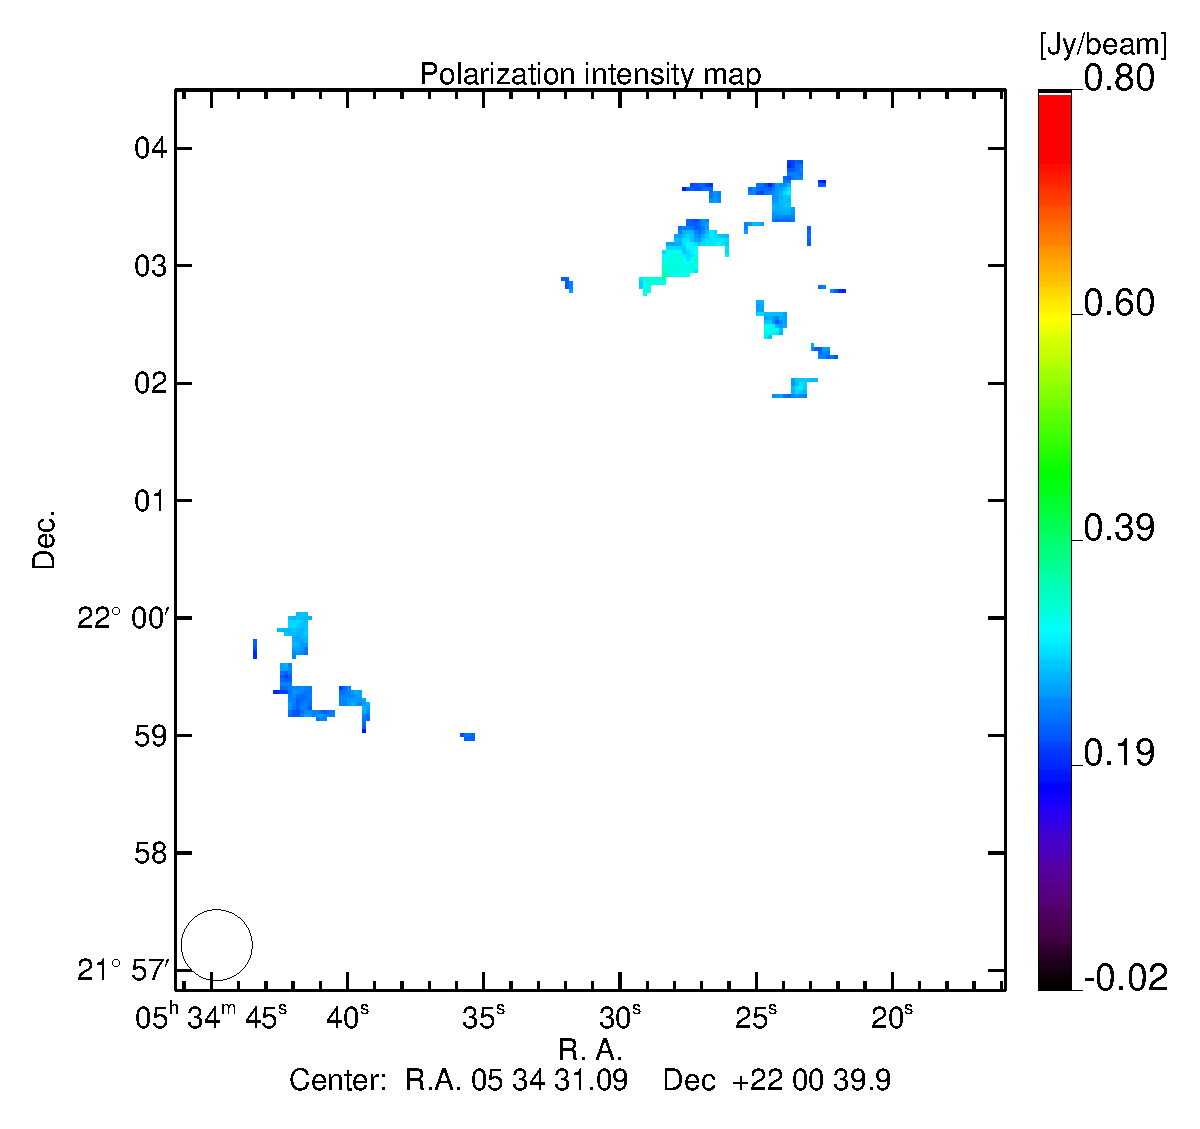
\includegraphics[width=0.75\linewidth,keepaspectratio]{figures/Crab_ipol2_2mm.pdf}}
\caption{\NIKA\ Polarization intensity map of the  Crab nebula at 150 GHz. The map shows high polarized emission reaching a value of 0.8 Jy beam$^{-1}$.}
\label{crab_ipol_maps}		
  \end{figure}
 

\section{\NIKA\ observations of the Crab Nebula}\label{sec:NIKA observations}
\subsection{\NIKA\ camera and polarization setup}\label{sec:nika camera}
\NIKA\ is a dual band camera observing the sky in intensity and polarization at 150 and 260 GHz with a FOV of 1.8$^{\prime}$, and 18$^{\prime\prime}$ and 12$^{\prime\prime}$ FWHM resolution, respectively. It has been operated at the IRAM 30 m telescope between 2012 and 2015. A detailed description of the \NIKA\ camera can be found in \citet{monfardini2010, monfardini2011} and \citet{catalano2014}. In addition to perform intensity observations \NIKA\ was also a test bench for polarization facilities of the final instrument \NIKAd, which was installed at the telescope in October, 2015 \citep{calvo2016,2016arXiv160508628C}.

The polarization setup of the NIKA camera consists of a continuously rotating room temperature metal mesh half wave plate (HWP) followed by an analyzer at room temperature, and polarization insensitive arrays of KIDs cooled down to 100 mK. The HWP rotation modulates the input polarization signal at four times the HWP rotation frequency allowing a quasi simultaneous measurement of the I, Q and U Stokes parameters.
%The characterization of the \NIKA\ polarization capabilities has been very important to get prepared for the follow-up camera \NIKA\. Beyondthat, 
\cite{ritacco2017} gives more details on the \NIKA\ polarization facilities and describes the performance of the instrument at the telescope. 
\NIKA\ has provided the first polarization observations performed with Kinetic Inductance Detectors, which represent a suitable detector technology for the development of the next generation of CMB experiments.
%Unfortunately, the observations of the Crab nebula performed at 260 GHz have been limited by the sensitivity of the \NIKA\ instrument in polarization and the resulting maps show a no significant detection, for that reason here we discuss only the observations performed at 150 GHz. 

\subsection{\NIKA\ observations}\label{sec:nika_observations}
%Polarization measurements with the \NIKA\ camera have been carried out with a combined action of a continuously rotating metal-mesh Half Wave %Plate (HWP), a polarizer and KIDs arrays mounted inside the \NIKA\ instrument. 
%Since \NIKA\ detectors \citep{roesch2012} are not sensitive to the linear polarization a polarizer is necessary to select one direction of it. 
Crab nebula polarization observations with the \NIKA\ camera were performed at the IRAM 30 m telescope during the observational campaign of February, 2015. Fig.~\ref{crab_intensity_maps} shows the Stokes $I$, $Q$ and $U$ maps obtained by a co-addition of 16 on-the-fly maps of 8 $\times$ 6 arcminutes for a total observation time of $\sim$ 2.7 hours. The maps were performed in equatorial coordinates according to four different scan directions: 0$^{\circ}$, 90$^{\circ}$, 120$^{\circ}$, 150$^{\circ}$. This allowed us to have the best covering of the source and to reduce
filtering effects.

To obtain the $I$, $Q$, and $U$ Crab nebula maps we have used a dedicated polarization data reduction pipeline \citep{ritacco2017}, which is an extension of the intensity \NIKA\ pipeline \citep{catalano2014,adam2013}. The main steps of the polarization pipeline are summarized below:
\begin{enumerate}
\item  Subtraction of the HWP induced parasitic signal, which is modulated at harmonics of the HWP rotation frequency and represents the most annoying noise contributing to the polarized signal. 
\item Reconstruction of the Stokes $I$, $Q$ and $U$ time ordered information (TOI) from the raw modulated data. This is achieved using a demodulation procedure consisting in a lock-in around the fourth harmonic of the HWP rotation frequency, where the polarization signal is located.
\item Subtraction of the atmospheric emission in the demodulated TOIs using decorrelation algorithms. In polarization the HWP modulation reduces significantly the atmospheric contamination. However simple common mode decorrelation methods can be used \citep{ritacco2017}. By contrast, in intensity the atmospheric emission fully dominates the signal and to recover the large angular scales we use the dual-band decorrelation algorithm presented in \cite{adam2013}.
%In order to have a proper estimate of the polarization degree we need to have a proper reconstruction of the intensity map. For an extended source like the Crab nebula, with angular size larger than the \NIKA\ FoV, it is difficult to correctly estimate its intensity emission avoiding filtering effects due to noise decorrelation methods. A common mode decorrelation method consisting on a template reconstruction (to be subtracted) using only the pixels outside the source is usually used in \NIKA\ data analysis. Filtering effects can be encountered in regions where the number of pixels used for the template reconstruction is too low.
%In order to avoid such an effect the Stokes $I$ map shown on the left panel of Fig.~\ref{crab_intensity_maps} has been obtained by using a decorrelation method called ``dual-band decorrelation''. Such a decorrelation algorithm has been developed for the reconstruction of the Sunyaev-Zel'dovich signal in galaxy clusters observations \citep{adam2013} taking advantage of \NIKA\ dual-band capabilities. The idea of this algorithm arises with the fact that the atmospheric emission is stronger at 260 GHz than at 150 GHz, as a consequence we can use 260 GHz observations as a ``template'' of the atmospheric emission to be subtracted to the 150 GHz observational data.


\item Projection of the demodulated and decorrelated Stokes I, Q, and U TOIs into Stokes I, Q and U maps.

\item Correction of the intensity to polarization leakage effect, which was identified on observations of unpolarized sources like the planet Uranus. For point sources the effect is about 3\% peak-to-peak, while for extended sources like the Crab nebula is of the order of 0.5 \% peak to peak. After correction the leakage effect in extended sources is negligible. 
%, and corrected by developing an algorithm able to reduce the effect from $\sim$ 3\% to lower than 1\%. More details on this effect and the data analysis pipeline can be found in \cite{ritacco2017}.
%For the Crab nebula observations the leakage systematic effect reaches a value of 0.5\% peak-to-peak of the total intensity.
%The level of this spurious instrumental polarization appears significantly lower on an extended source than on Uranus. 
%This can be due to a compensation of the negative and positive signal between adjacent pixels. Although the effect is weaker the algorithm of correction is still applied to obtain the final maps represented in Fig.~\ref{crab_intensity_maps}.
\end{enumerate}
% The first step of this dedicated module sees the subtraction of the a parasite signal which is modulated at harmonics of the HWP rotation %frequency and represents the most annoying noise contributing to the polarized signal. 
%The second step is the reconstruction of the Stokes $I$, $Q$ and $U$ time ordered information (TOI) from modulated data. This is achieved using a demodulation procedure consisting in a lock-in around the fourth harmonic of the HWP rotation frequency, where the polarization signal is located. 
%Finally, an intensity to polarization leakage effect was observed on the observation of an unpolarized source, the planet Uranus, and corrected by developing an algorithm able to reduce the effect from $\sim$ 3\% to lower than 1\%. More details on this effect and the data analysis pipeline can be found in \cite{ritacco2017}.
%For the Crab nebula observations the leakage systematic effect reaches a value of 0.5\% peak-to-peak of the total intensity.
%The level of this spurious instrumental polarization appears significantly lower on an extended source than on Uranus. 
%This can be due to a compensation of the negative and positive signal between adjacent pixels. Although the effect is weaker the algorithm of correction is still applied to obtain the final maps represented in Fig.~\ref{crab_intensity_maps}.

%In order to have a proper estimate of the polarization degree we need to have a proper reconstruction of the intensity map. For an extended source like the Crab nebula, with angular size larger than the \NIKA\ FoV, it is difficult to correctly estimate its intensity emission avoiding filtering effects due to noise decorrelation methods. A common mode decorrelation method consisting on a template reconstruction (to be subtracted) using only the pixels outside the source is usually used in \NIKA\ data analysis. Filtering effects can be encountered in regions where the number of pixels used for the template reconstruction is too low.
%In order to avoid such an effect the Stokes $I$ map shown on the left panel of Fig.~\ref{crab_intensity_maps} has been obtained by using a decorrelation method called ``dual-band decorrelation''. Such a decorrelation algorithm has been developed for the reconstruction of the Sunyaev-Zel'dovich signal in galaxy clusters observations \citep{adam2013} taking advantage of \NIKA\ dual-band capabilities. The idea of this algorithm arises with the fact that the atmospheric emission is stronger at 260 GHz than at 150 GHz, as a consequence we can use 260 GHz observations as a ``template'' of the atmospheric emission to be subtracted to the 150 GHz observational data.
 


 %The level of this spurious instrumental polarization is significantly lower than the observed one on Uranus. This is probably due to a compensation of the negative and positive signal between adjacent pixels. Although the leakage effect is very weak on this diffuse source the correction is still applied to produce the final maps presented in Fig.~\ref{crab_intensity_maps}.


%This data analysis allows to produce Stokes $I$, $Q$ and $U$ maps as shown in Figg.~\ref{crab_intensity_maps},\ref{crab_polarization_maps}. The continuos rotation of the HWP running at 2.98 Hz permits to shift the polarized signal at higher frequencies. In this way the polarized signal is cleaned by the low frequency noise (e.g.~atmosphere variations, electronics etc), but the intensity signal could be. As a consequence an accurate determination of the polarization fraction requires a good estimation of the total intensity map. 

%Fig.~\ref{crab_intensity_maps} shows the Stokes intensity map obtained at 150 GHz using the dual band decorrelation method.


%For illustration we show in Fig.~\ref{fig:crab_leakage_maps} the intensity to polarization leakage maps of Stokes $Q$ and $U$ of the Crab nebula, obtained as subtraction of the $Q$ and $U$ maps before and after leakage correction.

%\begin{figure}[h!]
%\begin{center}
%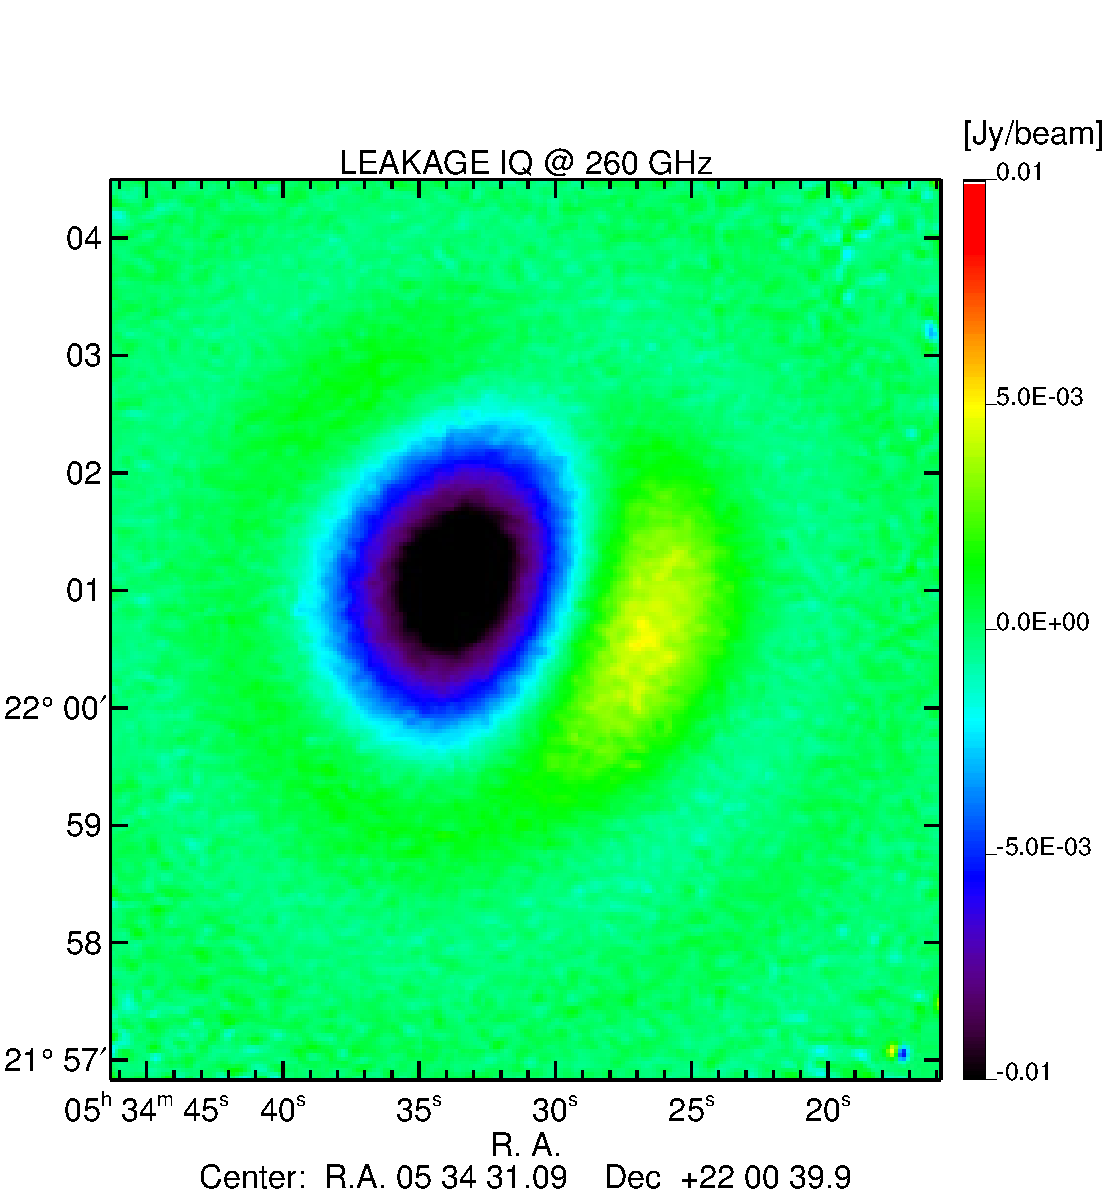
\includegraphics[clip, angle=0, scale = 0.23]{figures/Crab_IQ_1mm.pdf}
%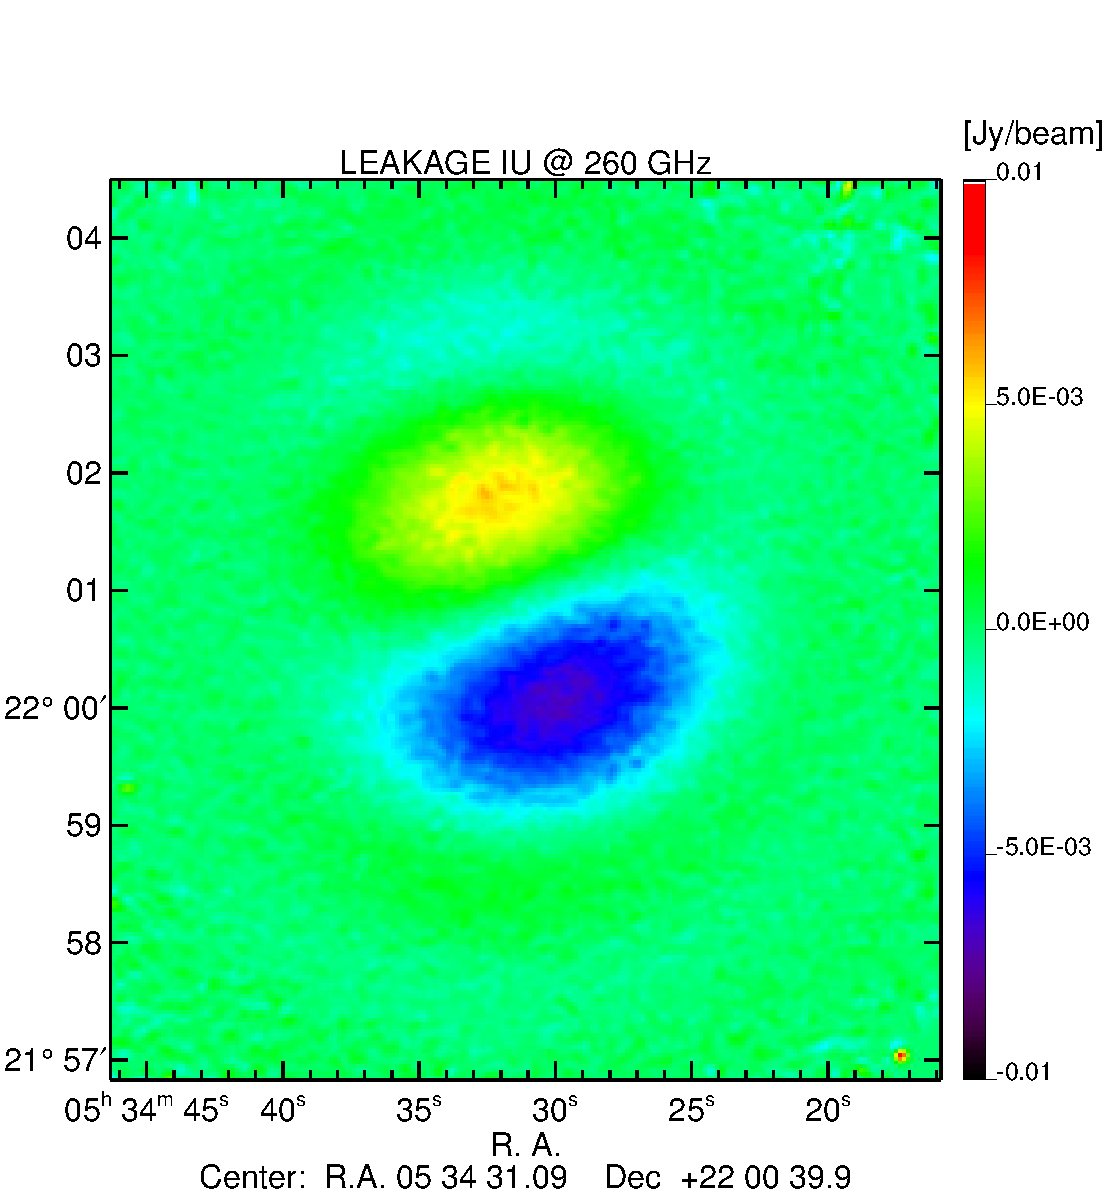
\includegraphics[clip, angle=0, scale = 0.23]{figures/Crab_IU_1mm.pdf}

%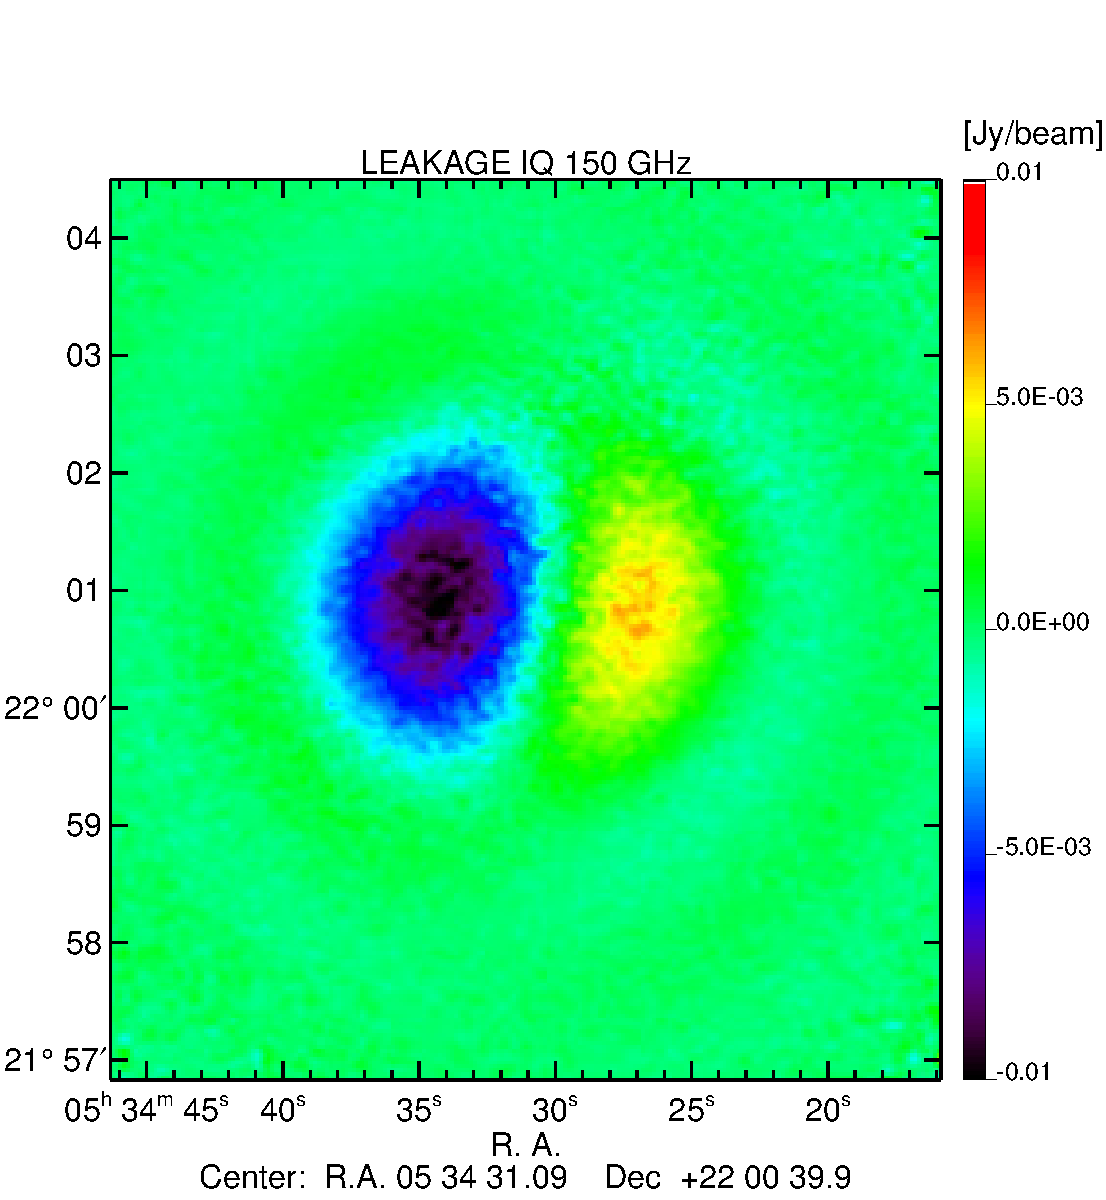
\includegraphics[clip, angle=0, scale = 0.23]{figures/Crab_IQ_2mm.pdf}
%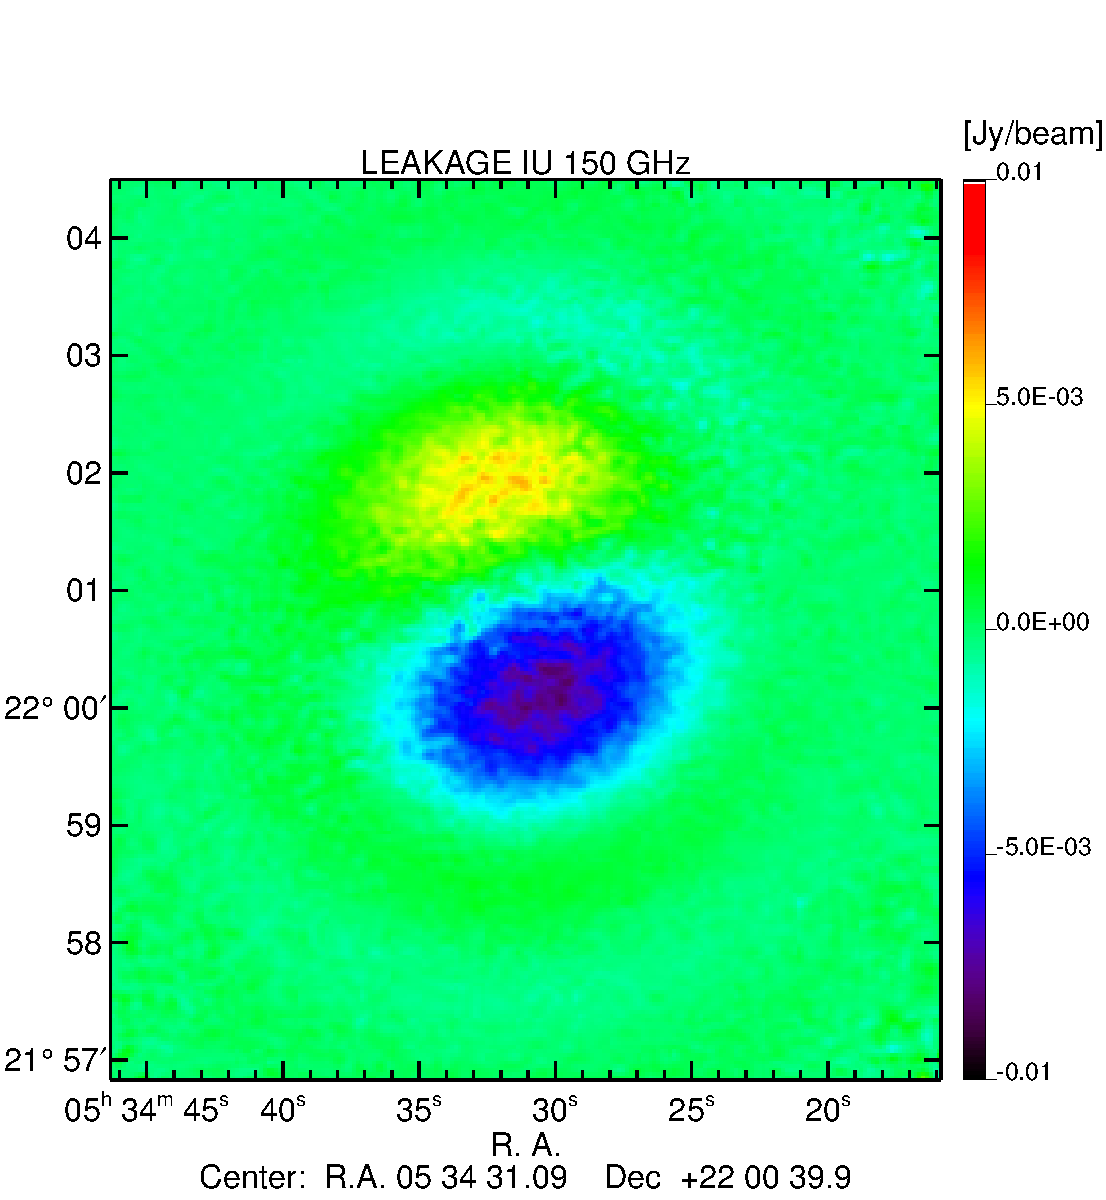
\includegraphics[clip, angle=0, scale = 0.23]{figures/Crab_IU_2mm.pdf}
%\caption{Crab Nebula Stokes $Q$ and $U$ intensity to polarization leakage maps. The peak-to-peak estimation reaches a value 0.5\% of the total intensity emission, respectively. See the total intensity map represented in Fig.~\ref{crab_intensity_maps}.}
%\label{fig:crab_leakage_maps}
%\end{center}
%\end{figure}

%The intensity to polarization leakage peak-to-peak reaches a value of $\sim$ 1\% (260 GHz) and 0.5\% (150 GHz) of the total intensity, see Fig.~\ref{fig:crab_leakage_maps}. 

\subsection{Crab polarization properties}\label{sec:pol_properties}
In this section we discuss the polarization properties of the source in terms of polarization degree $p$ and angle $\psi$, which are defined through the Stokes parameters $I, Q$, and $U$ as follows:
\begin{equation}
 p    = \frac{\sqrt{Q^2 + U^2}}{I} \nonumber 
\end{equation}
and
 \begin{equation}
 \psi = \frac{1}{2}\arctan\frac{U}{Q}.\label{angledegree_polar}
 \end{equation}
These definitions are not linear in $I$, $Q$ and $U$ and are noise biased. 
\citet{1980A&A....91...97S,1985A&A...142..100S,montier} proposed analytical solutions to correct this bias. At the limit of high S/N ratio the polarization degree and its uncertainties reads:
 \begin{eqnarray}
 p    &=& \frac{\sqrt{Q^2 + U^2 - \sigma_{Q}^2 - \sigma_{U}^2}}{I}, \nonumber \\ 
  \sigma_{p} &=& \frac{\sqrt{Q^2\sigma_Q^2 + U^2\sigma_U^2 + p^4I^2\sigma_I^2}}{pI^2}.
  \label{p_true_degree}
 \end{eqnarray}
 Furthermore, the polarization angle in a high S/N regime can be approximated by Eq.~\ref{angledegree_polar} with uncertainty
  \begin{eqnarray}\label{angle_uncertainty}
  \sigma_{\psi} = \frac{\sqrt{Q^2\sigma_Q^2 + U^2\sigma_u^2}}{2(pI)^2}.
  \end{eqnarray}

The polarization degree $p$ spatial distribution of the Crab nebula without noise bias correction is presented on the top left panel of Fig.~\ref{fig:pol_degree}. The polarization reaches 35 \% of the intensity across the intensity peak and decreases when moving towards the edges of the source. 
This feature highlights the interest of high resolution polarization observations of the Crab nebula. The top right panel of the figure shows the polarization degree $p$ as function of the total intensity map. Here the polarization degree values have been noise bias corrected and satisfy the condition P=$\sqrt{Q^2+U^2}$ $\textgreater$ 5 $\sigma_P$. The distribution of the polarization degree appears highly dispersed around a mean value of 20\%.

The bottom left panel of Fig.~\ref{fig:pol_degree} shows  the polarization angle, $\psi$, spatial distribution.
We observe a relatively constant polarization angle, about 150 $^{\circ}$ represented here in equatorial coordinates, except for the northern region where the averaged angle is around $220^{\circ}$, and some inner regions with lower polarization angle.
These values are confirmed by the bottom right panel that shows the polarization angle distribution as a function of total intensity satisfying the condition P=$\sqrt{Q^2+U^2}$  $\textgreater$ 5 $\sigma_P$.

The sudden change of polarization angle on the northern region was already observed by the XPOL experiment at 90 GHz \citep{aumont2010}.
This together with the variation of the polarization fraction discussed above confirms the need of high angular resolution observations at low and high frequencies for a good understanding of the Crab polarized emission proprieties.

We present in Fig.~\ref{crab_ipol_maps} the 150 GHz Crab polarization intensity map $P$. We observe a peak at 0.8 Jy beam$^{-1}$ and the polarization decreases towards the edges of the nebula.

%The polarization intensity $P$ map, represented in Fig.~\ref{crab_ipol_maps}, exhibits a polarized emission peaked at 0.8 Jy beam$^{-1}$ and decreasing to 0.1 Jy beam$^{-1}$ on the extremities of the nebula. 

\section{Total intensity and polarization fluxes}\label{sec:Polarization estimates in CMB experiments like beams}
We compute the total intensity flux across the Crab nebula, which has an extension of about  4$^{\prime}$ as shown in Fig.~\ref{crab_intensity_maps}.
We use standard aperture photometry techniques to calculate the flux as shown in Fig.~\ref{crab_integrated_flux}. We use as center position the center of the map. A zero level in the map, calculated as the mean of the signal measured on an external annular ring region 4$^\prime$ $\textless$  R $\textless$ 4.5$^\prime$, has been subtracted from the map. The total signal estimated is 204.4$\pm$7.9$\pm$10.2 Jy. The first uncertainty term accounts for statistical uncertainties computed from fluctuations of the signal at large radii. The second term corresponds to calibration errors estimated to $\simeq$ 5\% at 150 GHz. This absolute calibration error is obtained from the dispersion of the estimated flux of Uranus for observations collected during the same observational campaign \citep{ritacco2017}.

\begin{figure}[h!]
  \centering
     { 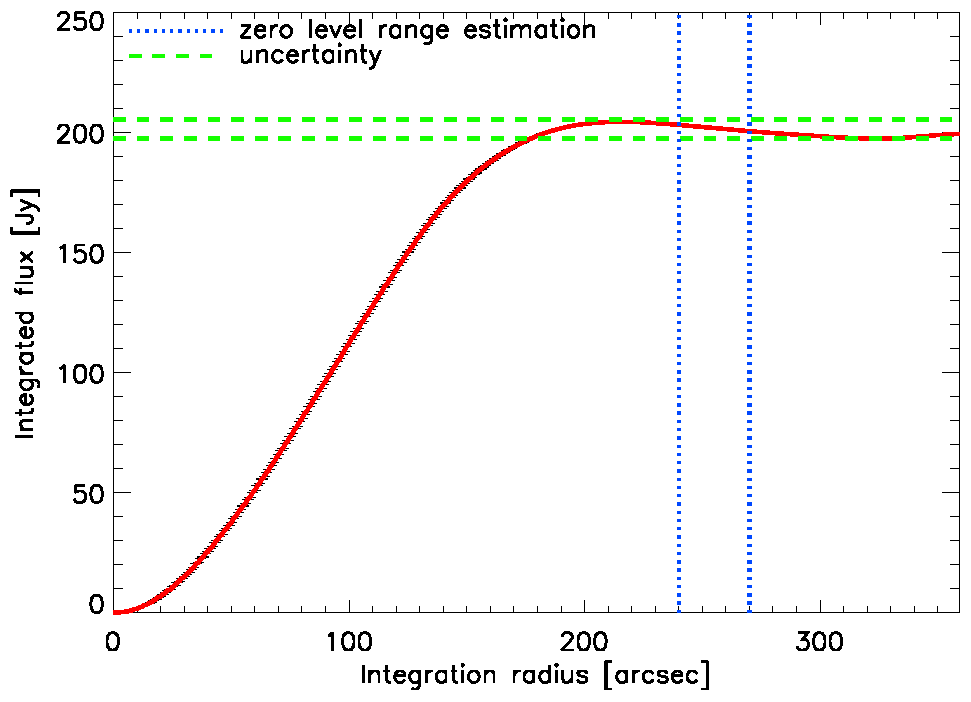
\includegraphics[width=0.85\linewidth,keepaspectratio]{figures/Crab_integrated_flux_2mm.pdf}}
     \caption{Cumulative flux of the Crab nebula at 150 GHz. The flux has been corrected by a zero level in the map, which corresponds to the mean of the signal calculated in an annular ring as indicated by the blue dotted lines. The green dotted line represents the uncertainties measured at large radii.}
\label{crab_integrated_flux}
\end{figure}

For comparison with low angular resolution CMB experiments we also give the polarization degree $p$ and angle $\psi$ integrated values obtained in well defined regions: 5$^\prime$, 7$^\prime$ and around the peak of intensity.
Tab.~\ref{tab:crab_results} shows the total intensity $I$, polarized intensity $P$, polarization degree $p$ and polarization angle $\psi$ obtained in three different regions. 
%To compare with the \Planck\ satellite we estimate the values in two regions of $7^{\prime}$ and $5^{\prime}$ width corresponding to the beam widths of the \Planck\ frequency channels at 143 and 217 GHz, respectively. 
%Further, two other regions are defined at high S/N ratio: where $P$ $\textgreater$ $3\sigma_P$ and  where $P$ $\textgreater$ 0.2 Jy. 
Notice that the polarization angles are represented in Galactic coordinates to ease the comparison with the \Planck\ \citep{2015arXiv150702058P} and \WMAP\ CMB experiments \citep{2011ApJS..192...19W}. 

Fig.~\ref{crab_p_angle_comparison} shows the polarization fraction (top) and angle (bottom) of the Crab nebula as function of the frequency as measured by five different instruments: \Planck\ \citep{2015arXiv150702058P}, \WMAP\ \citep{2011ApJS..192...19W}, XPOL \citep{aumont2010}, SCUPOL \citep{scubapol} and \NIKA\ (this paper).
For \NIKA\ we have averaged within a 5$^\prime$ region and considered only pixels for which $P$ $\textgreater$ $3\sigma_P$. 
%Notice that SCUPOL maps \citep{scubapol} provided at 352 GHz have reduced angular size w.r.t \NIKA. In order to compare with it we define a small region of 1.4$^\prime$ around the peak of the polarization intensity. 
%For the polarization fraction we keep the convention used by XPOL \citep{aumont2010} and we represent in the figure the value measured within 5$^{\prime}$. 
The solid line in both figures represents the mean value found using all the observations shown and the dashed lines represent the standard deviation. 

\begin{table*}
  \centering
      \begin{tabular}{ccccccccc}
      \hline
      \hline
       & $I$ & $P$ & $p$ & $\psi$  \\ 
                                         & [Jy]         &    [Jy]         & [\%]  & [$^\circ$] \\
      \hline
      \hline
 %seen by 7$^{\prime}$   & 231.8$\pm$0.2  & 14.03$\pm$0.09 & 6.05$\pm$0.04 & -85.1$\pm$0.5$\pm$1.8(syst)  \\ 
   seen by 7$^{\prime}$   & 231.8$\pm$0.2  & 14.03$\pm$0.09 & 6.05$\pm$0.04 & -87.14$\pm$0.07$\pm$1.8(syst)  \\ 
 
%            seen by 5$^{\prime}$ & 219.0$\pm$0.1  & 14.8 $\pm$0.03 & 6.78$\pm$0.01 & -83.7$\pm$0.1$\pm$1.8(syst)    \\ 
          seen by 5$^{\prime}$ & 219.0$\pm$0.1  & 14.8 $\pm$0.03 & 6.78$\pm$0.01 & -87.15$\pm$0.04$\pm$1.8(syst)    \\ 
  %    P $\textgreater$ 3 $\sigma_P$     & 84.6$\pm$0.01  & 10.51 $\pm$0.01 &12.42$\pm$0.01 & -87.15 $\pm$0.04$\pm$1.8(syst) \\
     	      
              seen by 1.4$^{\prime}$ with P $\textgreater$ 0.2 Jy& 60.6$\pm$0.2 & 10.28$\pm$0.01  & 16.96$\pm$0.01 &-87.69$\pm$0.01$\pm$1.8(syst)\\
              
             
                \hline            
    \hline   
    \end{tabular}
   \caption{ Total intensity flux $I$ and  polarized intensity flux, $P$, polarization degree $p$, and angle $\psi$. The values have been calculated in regions with high S/N and within 7$^{\prime}$, 5$^{\prime}$ from the center of the source and around the peak of intensity. An absolute calibration error of 5 $\%$ must be accounted for and propagated to the polarization estimates. A polarization angle systematic uncertainty of 1.8$^{\circ}$ is also considered.
   The polarization angle estimation satisfies the condition P $\textgreater$ 3$\sigma_P$ to avoid noise bias. 
   %The values measured in two regions with high S/N ratio are also presented.
    }
    \label{tab:crab_results}
 \end{table*}
  

\begin{figure}
  \centering
          { 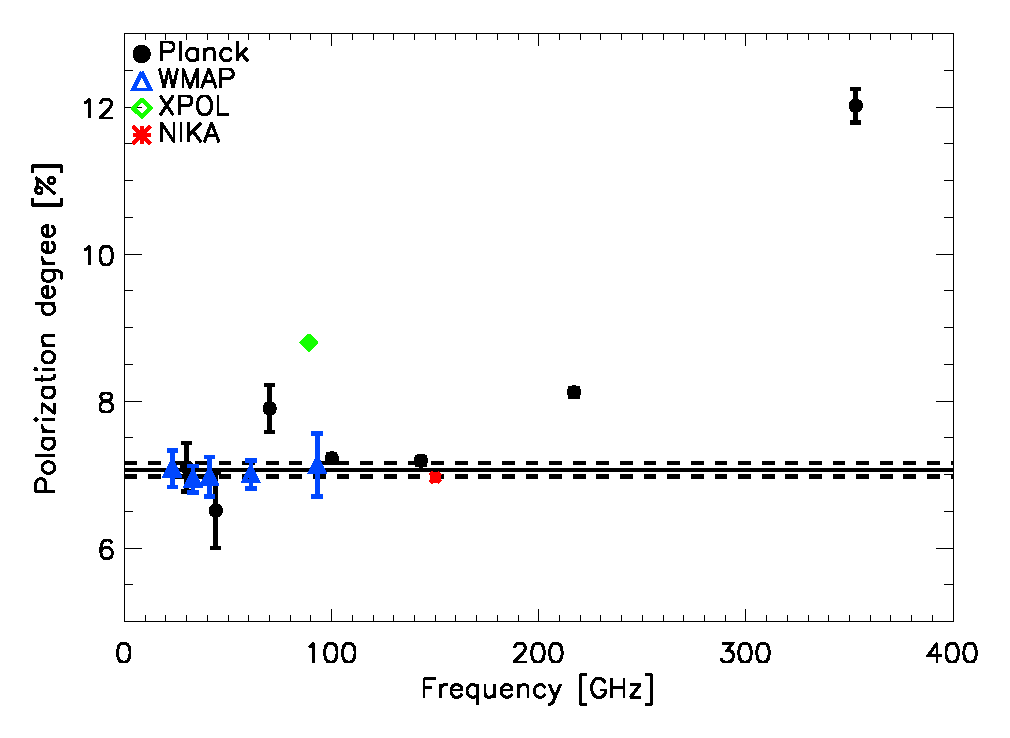
\includegraphics[width=1\linewidth,keepaspectratio]{figures/pdegree_comparison.pdf}}
          { 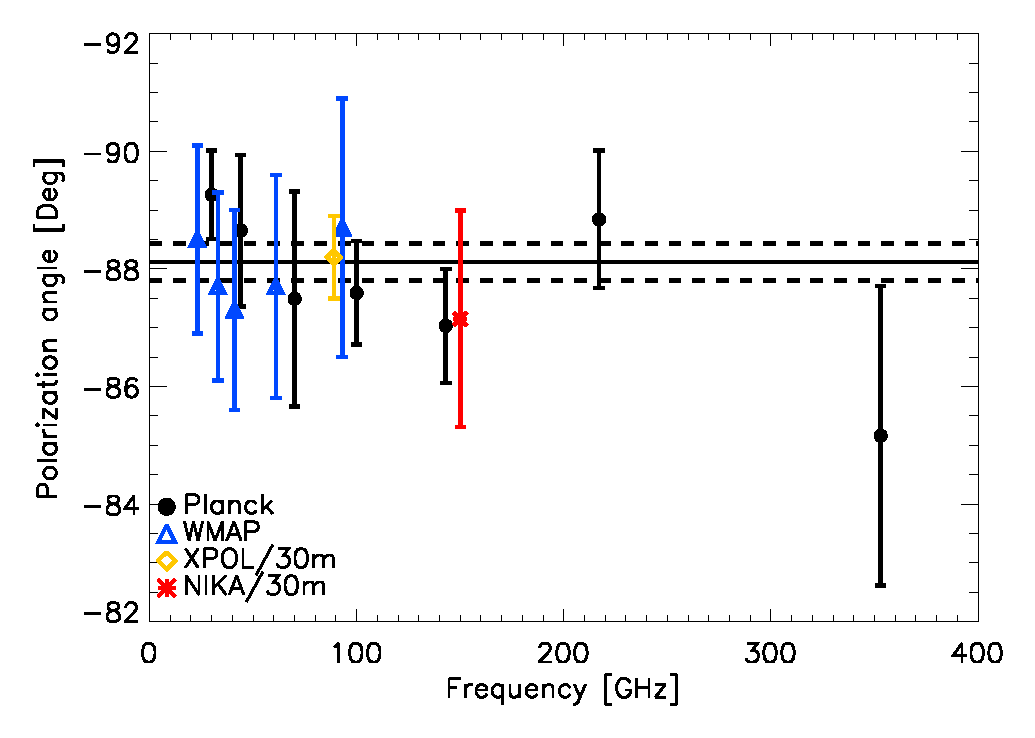
\includegraphics[width=1\linewidth,keepaspectratio]{figures/angle_comparison.pdf}} 
            \caption{{\it Top}: polarization degree as a function of frequency as measured by \Planck\ (black dots), WMAP (blue triangles), XPOL (green diamond), SCUPOL (cyan cross) and \NIKA\ (red crosses). The \NIKA\ value has been estimated by integrating in a radius of $5^{\prime}$ as given by XPOL \citep{aumont2010}. The solid line represents the weighted-average degree of polarization accounting for low frequency values (\textless 200 GHz) and excluding XPOL.
            Dashed lines are the uncertainties.
            {\it Bottom}: polarization angles in Galactic coordinates for the same five experiments given above. The solid line represents the weighted-averaged polarization angle accounting for all observations but SCUPOL and dashed lines are the uncertainties.
Notice that SCUPOL values \citep{scubapol} at 352 GHz have been estimate on maps covering only a region of 1.4$^\prime$ across the source.}
\label{crab_p_angle_comparison}		
  \end{figure}

%\begin{table*}
 % \centering
  %    \begin{tabular}{ccccccccc}
  %    \hline
  %    \hline
  %     Experiments & Frequency & $\psi$ & $p$ & Comments \\ 
  %                                      & [GHz]  & [$^\circ$] & [\%] & \\
  %   \hline
  %   \hline
  %   \NIKA\ &  150 & -87.15 $\pm$ 0.01 (stat) $\pm$ 1.8 (syst) & 6.97$\pm$0.04 & This paper\\
  %  \Planck\ & 143 & -87.03 $\pm$ 0.97 & 7.19 $\pm$ 0.05 & \citep{2015arXiv150702058P} \\
  %   XPOL & 90 & -88.2 $\pm$ 0.7 & 8.8 $\pm$ 0.02 & \citep{aumont2010} \\
  %   \WMAP\ & 94 & -88.7 $\pm$ 2.2 & 7.13 $\pm$ 0.43 & \citep{2011ApJS..192...19W} \\
  %  \hline
  %  \hline   
  %  \end{tabular}
  %  \caption{Polarization angle and degree results obtained by four different experiments. For \NIKA\ and XPOL we estimate the values in five arcmin angular size, which corresponds to the beam of \Planck\ and \WMAP\ at 143 and 94 GHz, respectively.}
  %  \end{table*}
Considering only low frequency data (\textless 200 GHz) and excluding the XPOL data (see below) we find that the degree of polarization of the Crab nebula at arcmin scales is 7.1$\pm$0.1 \%.
In terms of degree of polarization most data sets are consistent at 2$\sigma$ level with the weighted-average value. For XPOL the discrepancy can probably be explained by a relatively low intensity flux with respect to the other experiments, which tends to increase the polarization fraction. In the case of \Planck\ the discrepancy observed at high frequency may be due to an evolution with frequency of the Crab nebula polarization properties.
However, this hypothesis is disfavored by the polarization
angle measurements that seems to be consistent with the mean value across all frequencies but for the SCUPOL data. The latter can be understood in terms of spatial variations as SCUPOL has only observed a 1.4$^\prime$ region around the peak in polarization intensity. 
The weighted-average of the polarization angle of the Crab nebula at arcmin scales, which was estimated considering all available observations but SCUPOL, is -88.1 $\pm$ 0.3.
All the observations shown on the bottom panel of Fig.~\ref{angledegree_polar} agree within 1$\sigma$ with this value except for the \Planck\ value at 30 GHz, which is slightly high. 

\section{Crab Spectral Energy Distribution in intensity and polarization}\label{sec:Polarization intensity Spectral Energy Density (SED)}
\subsection{Intensity}
The total intensity emission of the Crab nebula at radio and millimeter wavelengths (1 and 500 GHz) is mainly due to synchrotron emission and can be well described by a single power law of the form:

\begin{equation}
I_{\nu} = A(\nu / 1 GHz)^{\beta}
\end{equation}\label{eq:sync}
 with spectral index $\beta$ = -0.296$\pm$0.06 \citep{baars1977absolute,macias2010}. Further, the Crab nebula is fading with time at a rate of $\alpha$ = 0.167$\pm$0.015 \% yr$^{-1}$ \citep{aller1985decrease}. 
These results suggest a low frequency emission produced by particles accelerated by the same magnetic field. The direction of the polarization is thus expected to be constant across frequencies while the polarization degree may vary. 

We show in Fig.~\ref{crab_SED} the intensity flux of the Crab nebula as a function of frequency. The fluxes in the radio domain were taken from \cite{dmitrenko1970absolute} and \cite{1971IzVUZ..14..157V}. We also show microwave and mm wavelengths fluxes from \Archeops\ \citep{macias2007archeops}, \Planck\ \citep{2015arXiv150702058P}, WMAP \citep{2011ApJS..192...19W} and MAMBO \citep{2002A&A...386.1044B}. The measured \NIKA\ intensity flux at 150 GHz is shown in red.
We also present in the figure the best-fit to the data computed by $\chi^2$-minimization using observations below 100 GHz (cyan line). The amplitude and spectral index found are: 

\begin{equation}
 A = 980.6 \pm 0.7  ,\quad \beta = -0.3151 \pm 0.0002. 
 \end{equation}
 For illustration we also show the best-fit to the data found by \cite{macias2010} in a previous analysis (green line). 
Notice that fading is accounted for in the best-fit model as well as in the data presented in the figure.
The estimated best-fit model from this paper is a slightly different w.r.t the previous analysis mainly due to the addition of recently published results by \Planck\ \citep{2015arXiv150702058P} and  WMAP \citep{2011ApJS..192...19W}. However, the result found at 150 GHz by the \NIKA\ camera agrees at 1 $\sigma$ level with both models. 
Notice that, as discussed before, the XPOL intensity flux is low with respect to expectations from the two power law models. 
 
The \Planck\ data at 100, 143, 217 and 353 GHz seems to suggest another emission component in the Crab nebula. The break in the spectrum observed at around 90 GHz   suggest that another population of electrons contributes to the intensity emission. By contrast,  the results obtained by {\it Archeops}, MAMBO and \NIKA\ do not seem to support with this conclusion. 
To account for this break in the SED we assume a two power-laws model:
\begin{equation}
I_{\nu} = A(\nu/1GHz)^{\beta} \quad for \quad \nu   \textless  100 GHz
\end{equation}
and 
\begin{equation}
I_{\nu} = A_{H}(\nu/1GHz)^{\beta_H} \quad for \quad \nu   \textgreater  100 GHz
\end{equation}
By $\chi^2$-minimization we find
A$_H$ = 8.6 $\pm$ 0.45 and $\beta_H$ = -0.71 $\pm$ 0.09.
We note that the \NIKA\ data is consistent with this model at the 2$\sigma$ level. More data at the mm range is need to better understand the observed break of the SED at about 90 GHz. 


\subsection{Polarization}
The total intensity of the Crab nebula has been monitored along decades across a large range of frequency by contrast the amount of polarization observations is really poor.
Recent results provided by \Planck\ \citep{2015arXiv150702058P}, \WMAP\ \citep{2011ApJS..192...19W} and XPOL \citep{aumont2010} together with \NIKA\ allow us to trace the Crab nebula polarization intensity SED as shown in Fig.~\ref{crab_SED_ipol}. 
From the figure we observe that the data are not consistent with a single power law model as for intensity. 
The \Planck\ data show an oscillating SED while the \WMAP\ ones are more consistent with a power law model.
To investigate this issue further we assume a power law model for the data as discussed by the Eq.~\ref{eq:sync} and fit separately the \Planck\ and \WMAP\ data.
We restrict the fit to the data with $\nu \textless$ 100 GHz. We show in Fig.~\ref{crab_SED_ipol} in black and blue the best-fit model for the \Planck\ and \WMAP\ data, respectively.

Accounting for fading the fitted amplitude and spectral indexes $\beta$ are:
\begin{itemize}
\item best-fit parameters for \WMAP\ only data:
\begin{equation}
A = 78.9\pm7.8 \quad , \quad \beta_p = -0.35\pm0.03;
\end{equation}
\item best-fit parameters for \Planck\ only data:
\begin{equation}
A = 179.1\pm15.4 \quad , \quad \beta_p = -0.54\pm0.02.
\end{equation}
\end{itemize}

The \WMAP\ best-fit model is in agreement with \Planck\ observations at 30, 100 and 353 GHz.
The \Planck\ best-fit model seems to overestimate the polarization flux at low frequency. 
The \NIKA\ data at 150 GHz are consistent at the 1$\sigma$ level with the \WMAP\ and \Planck\ best-fit models.

We have also estimated the spectral index at high frequency using the map obtained by SCUPOL at 352 GHz (850 $\mu$m) and the \NIKA\ map. Considering only the region observed by SCUPOL we obtain:
\begin{equation}
\beta_p = -0.33 \pm 0.01.
\end{equation}

\begin{figure}
  \centering
          { 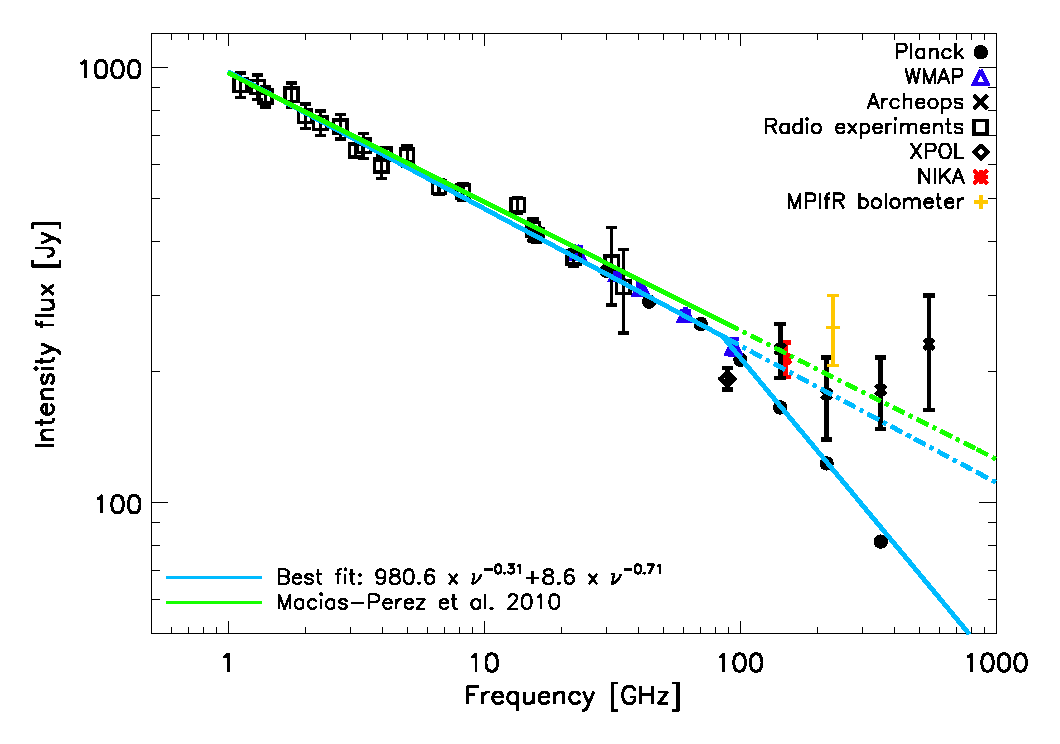
\includegraphics[width=1\linewidth,keepaspectratio]{figures/Crab_SED_i_150.pdf}}
           \caption{Crab nebula total intensity SED as obtained from \Planck\ \citep{2015arXiv150702058P}, \WMAP\ \citep{2011ApJS..192...19W}, Archeops \citep{macias2007archeops}, Radio experiments \citep{dmitrenko1970absolute, 1971IzVUZ..14..157V}, XPOL \citep{aumont2010}, \NIKA\ (this paper) and MAMBO \citep{2002A&A...386.1044B} data. The green line shows the model derived by a previous analysis discussed in \citep{macias2010}. The best-fit obtained by a new analysis is shown in cyan line. Both, the fit and the data account for the fading with the time.}
\label{crab_SED}		
  \end{figure} 

\begin{figure}
  \centering
             { 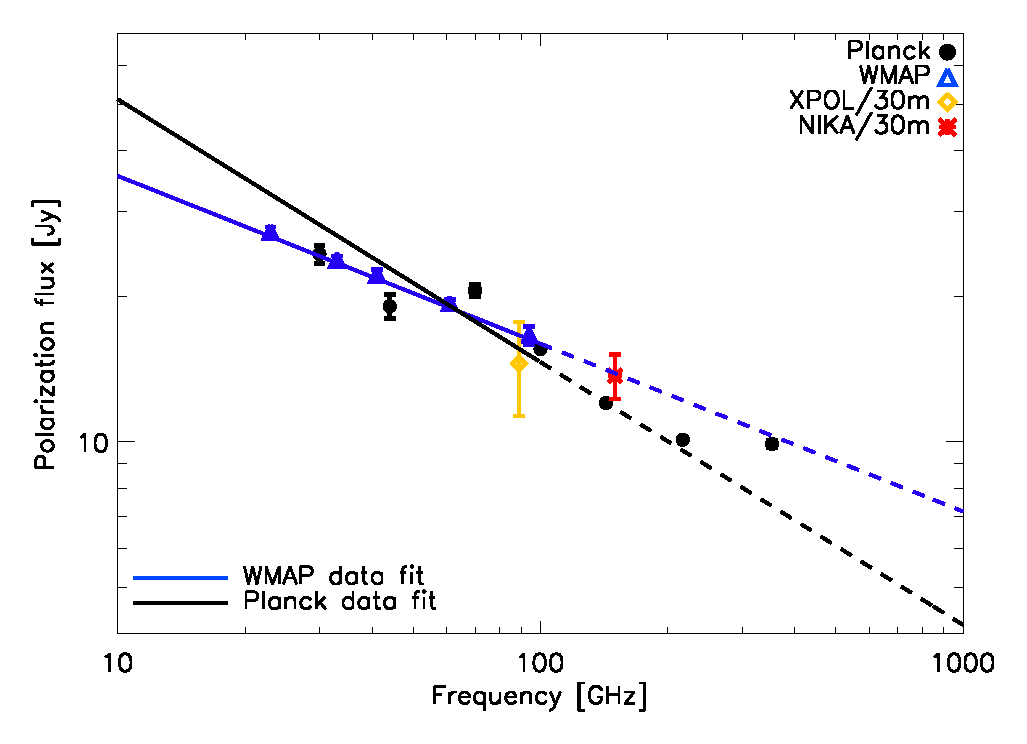
\includegraphics[width=1\linewidth,keepaspectratio]{figures/Crab_SED_ipol.pdf}}
           \caption{Crab nebula polarization intensity SED as obtained from the \Planck\ \citep{2015arXiv150702058P}, \WMAP\ \citep{2011ApJS..192...19W} and \NIKA\ (this paper) data. The two best-fit models presented have been estimated using only WMAP data (blu line) or \Planck\ data only (black line).}
\label{crab_SED_ipol}		
  \end{figure} 
 \noindent
This result is in good agreement with the \WMAP best-fit model spectral index.

%The left panel of Fig.~\ref{crab_beta_ipol} represents the spatial distribution of the spectral index $\beta$ where $I$ $\textgreater$ 3$\sigma$. $\beta$ is obtained as described by the Eq.~\ref{beta_equation} considering the \NIKA\ Stokes $I$ maps of Fig.~\ref{crab_intensity_maps} and accounting for the corresponding frequencies. 

%The right panel of Fig.~\ref{crab_beta_ipol} shows the total intensity map values at 260 GHz as function of the total intensity map observed at 150 GHz. The correlation found between the two frequencies suggests the same physical origin of the emission. 
%The value of the spectral index obtained by the fit is:
%\begin{equation}
%\beta = -0.482 \pm 0.002.
%\end{equation}
%The measured value is different from the expected spectral index from previous observation \citet{baars1977absolute,macias2010}. This difference can be explained by the noise decorrelation used, which is different for the two Stokes $I$ map estimation, that causes filtering effect on the map at 260 GHz.
%The measured spectral index is in agreement with what we observe on the map of the spatial distribution of $\beta$. Indeed, $\beta$ remains approximately constant around -0.45 in the most intense emission region of the source. The contours (red) represent the 150 GHz Stokes $I$ emission map. 

%\begin{figure*}[h!]
  %\centering
  %           { 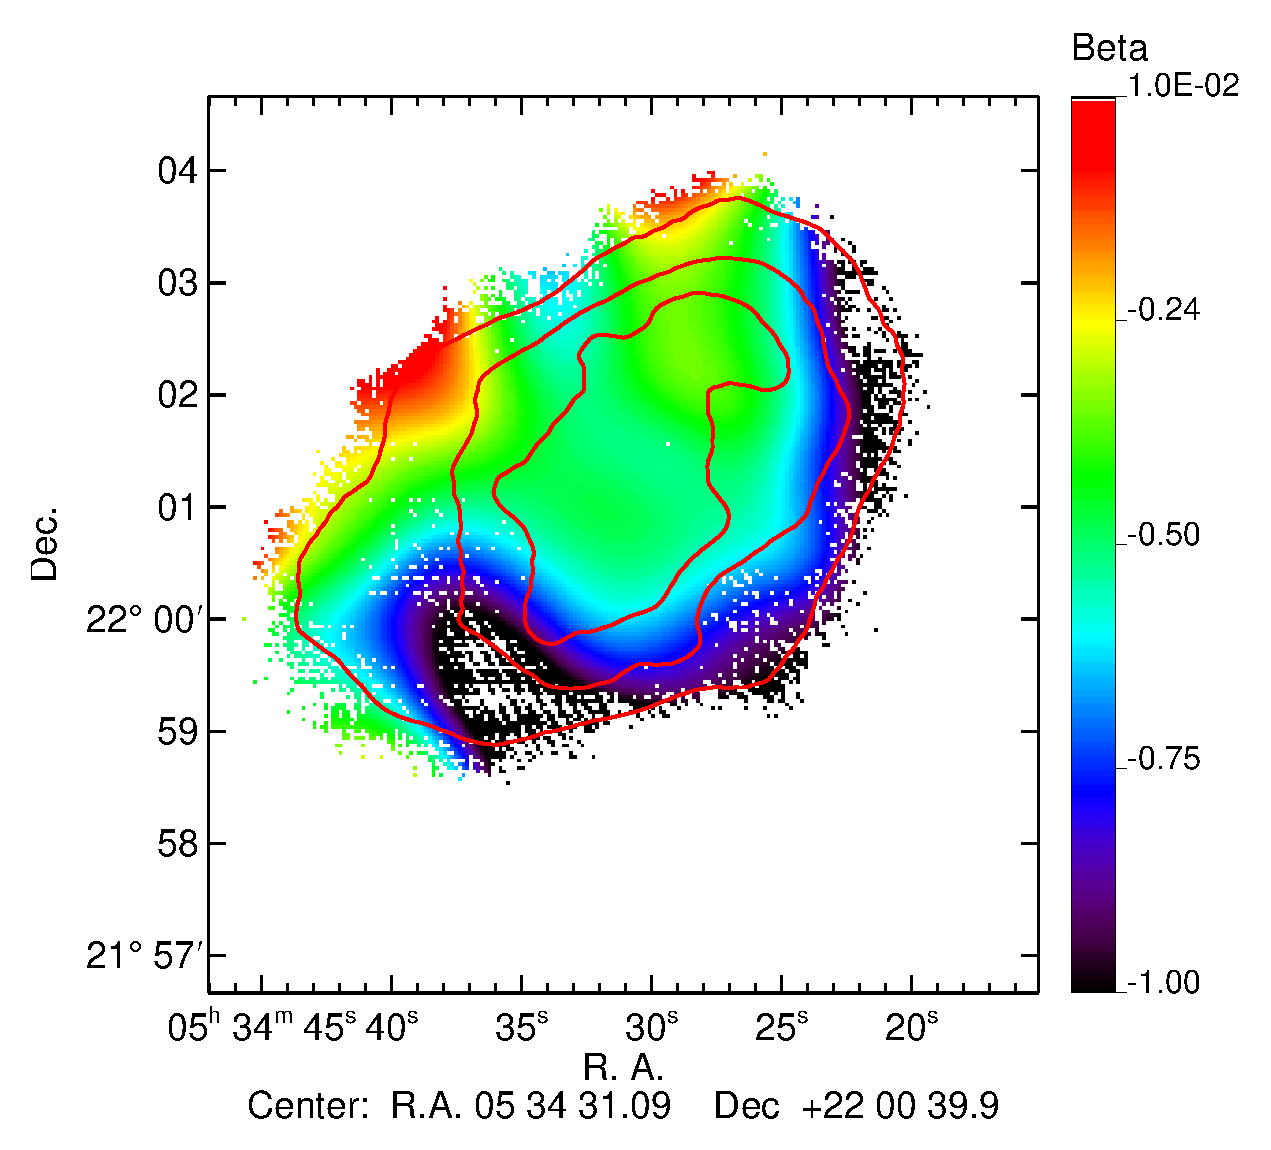
\includegraphics[width=0.4\linewidth,keepaspectratio]{figures/crab_beta_i.pdf}}
  %          { \includegraphics[width=0.5\linewidth,keepaspectratio]{figures/I_1mm_vs_2mm.pdf}}
  %        \caption{Spectral index map (left) obtained using the two NIKA total intensity maps. The correlation between the two maps is shown on the right panel.}
%\label{crab_beta_ipol}		
%  \end{figure*} 
%\subsection{Polarization spectral index}
%In polarization the low S/N observed at 260 GHz prevents us to have a significant detection and to derive the spatial distribution of the spectral index.



\section{Conclusions}\label{sec:conclusions}
The Crab nebula is considered an absolute calibrator for CMB experiments in terms of polarization degree and angle. This absolute calibration is particularly important for the measurement of the CMB polarization B-modes, which are a window which the \NIKA\ camera towards the physics of the early Universe.

We have reported in this paper first high resolution polarization measurements of the Crab nebula at 150 GHz. These observations has allowed us to accurately map the spatial distribution of the polarization fraction and angle. 
We find an averaged polarization angle of -87.15$\pm$0.04$\pm$1.8 within a region of 5$^\prime$ with respect to the central coordinates R.A.: 05$^{h}$ 34$^{m}$ 31.09 s, Dec.: +22$^{\circ}$ 00$^{\prime}$ 39.9$^{\prime\prime}$.
This is consistent with previous measurements from \Planck, \WMAP, and XPOL.

Using all available data sets in polarization to date we conclude that the polarization angle of the Crab nebula is consistent with being constant across frequencies, from 23 GHz to 217 GHz, at arcmin scales with a value of -88.1$\pm$0.3. 

We have characterized the intensity and polarization SED of the Crab nebula. 
In intensity recent \Planck\ data show a break in the SED suggesting the existence of two different popularion of electrons. In polarization we find that the data are overall consistent with a single power law spectrum as expected from synchrotron emission. However, we find some discrepancies between data sets, which will require further mm measurements at high resolution for a better understanding of the physics at play. 

\vspace{0.2cm}
 \begin{acknowledgements}
We would like to thank the IRAM staff for their support during the \NIKA\ campaigns. 
The NIKA dilution cryostat has been designed and built at the Institut N\'eel. 
In particular, we acknowledge the crucial contribution of the Cryogenics Group, and 
in particular Gregory Garde, Henri Rodenas, Jean Paul Leggeri, Philippe Camus. 
This work has been partially funded by the Foundation Nanoscience Grenoble, the LabEx FOCUS ANR-11-LABX-0013 and 
the ANR under the contracts ``MKIDS'', ``NIKA'' and ANR-15-CE31-0017. 
This work has benefited from the support of the European Research Council Advanced Grant ORISTARS 
under the European Union's Seventh Framework Programme (Grant Agreement no. 291294).
We acknowledge fundings from the ENIGMASS French LabEx (R. A. and F. R.), 
the CNES post-doctoral fellowship program (R. A.),  the CNES doctoral fellowship program (A. R.) and 
the FOCUS French LabEx doctoral fellowship program (A. R.).
\end{acknowledgements}


\bibliography{bib_crab.bib}


\end{document}
